\documentclass[xcolor=dvipsnames]{beamer}

\makeatletter


\usepackage{textcomp}%%needed for the euro symbol
\usepackage{mathpazo}%Letra palatino con fuentes para matemáticas
\usepackage[T1]{fontenc}
\usepackage[utf8]{inputenc}
\usepackage{graphicx}
\usepackage{url}
\usepackage{amsmath}
\usepackage{booktabs}

%\usepackage{epstopdf}


\usepackage[spanish]{babel}
\addto\shorthandsspanish{\spanishdeactivate{~<>}}



\hypersetup{pdfauthor={Oscar Perpi\~n\'an},%
    pdftitle={Energ\'ia Solar Fotovoltaica},%
    filecolor=blue,%
    urlcolor=blue}

\usepackage[emulate=units]{siunitx}
\sisetup{per=fraction, fraction=nice, decimalsymbol=comma}
\newunit{\wattpeak}{Wp}
\newunit{\watthour}{Wh}
\newunit{\amperehour}{Ah}

\setbeamercovered{transparent}
\setbeamertemplate{navigation symbols}{}
\usefonttheme{serif} 
\usefonttheme{structuresmallcapsserif} 

%\useinnertheme[shadow=true]{rounded}
%\useoutertheme{shadow}
\usecolortheme[named=OliveGreen]{structure} %sirve para cambiar el color genérico
\usefonttheme{structurebold}
%\usecolortheme{orchid}
%\usecolortheme{whale}
\usebackgroundtemplate{
\includegraphics[height=\paperheight]{../Figuras/LateralERMA.png}}
\logo{
\includegraphics[height=1cm]{../Figuras/LogoERMA.png}}

%\usepackage{mathpazo}%Letra palatino con fuentes para matemáticas
\usepackage[T1]{fontenc}
\usepackage[utf8]{inputenc}
\usepackage{graphicx}
\usepackage{url}
\usepackage{amsmath}
\usepackage{booktabs}
\usepackage{textcomp}%%needed for the euro symbol

\date{}

\usepackage[emulate=units]{siunitx}
\sisetup{per=fraction, fraction=nice, decimalsymbol=comma}
\newunit{\wattpeak}{Wp}
\newunit{\watthour}{Wh}
\newunit{\amperehour}{Ah}

\setbeamercovered{transparent}
\setbeamertemplate{navigation symbols}{}
\usefonttheme{structuresmallcapsserif} 
\usefonttheme{serif} 
\usefonttheme{structurebold}

%\usepackage{epstopdf}


\usepackage[spanish]{babel}
\addto\shorthandsspanish{\spanishdeactivate{~<>}}

\hypersetup{pdfauthor={Oscar Perpi\~n\'an},%
    pdftitle={Energ\'ia Solar Fotovoltaica},%
    filecolor=blue,%
    urlcolor=blue}



%\usepackage{handoutWithNotes} %para hacer papel con notas 
%\pgfpagesuselayout{4 on 1 with notes}[a4paper,border shrink=5mm]



%\usepackage{pgfpages}
%\pgfpagesuselayout{2 on 1}[a4paper,border shrink=5mm]




\makeatother

\begin{document}

\title{\textsc{Sistemas Fotovoltaicos }\\%
  \textsc{de Conexión a Red}}


\subtitle{Productividad, EPBT y Sombras}


\institute{Máster ERMA}


\date{}


\author{\textsc{Oscar Perpiñán Lamigueiro}\\%
  \url{http://oscarperpinan.github.io}}


\begin{frame}[plain]
  \titlepage
\end{frame}

\AtBeginSection[]{
    \begin{frame}[plain]
        \frametitle{Índice}
        %\setcounter{tocdepth}{1}
        \tableofcontents[currentsection] 
    \end{frame}
                  }

\selectlanguage{spanish}%

\section{Conceptos Generales}


\begin{frame}
\frametitle{SFCR sobre suelo}
\begin{itemize}
\item \textbf{Objetivo}: maximizar la producción energética anual del sistema
con el menor coste y la menor ocupación de terreno posibles
\item El diseñador debe configurar generador (tamaño y seguimiento) teniendo
en cuenta:

\begin{itemize}
\item \textbf{Inversión económica} (relacionada principalmente con la potencia
del generador)
\item \textbf{Rendimiento económico deseado} (relacionado con la energía
producida por el sistema y, por tanto, con el modo de seguimiento
empleado) 
\item \textbf{Ocupación de terreno} (relacionado con el modo de seguimiento
empleado).
\end{itemize}
\end{itemize}

\end{frame}

\begin{frame}[plain]
\frametitle{Estructuras sobre suelo}

\begin{center}
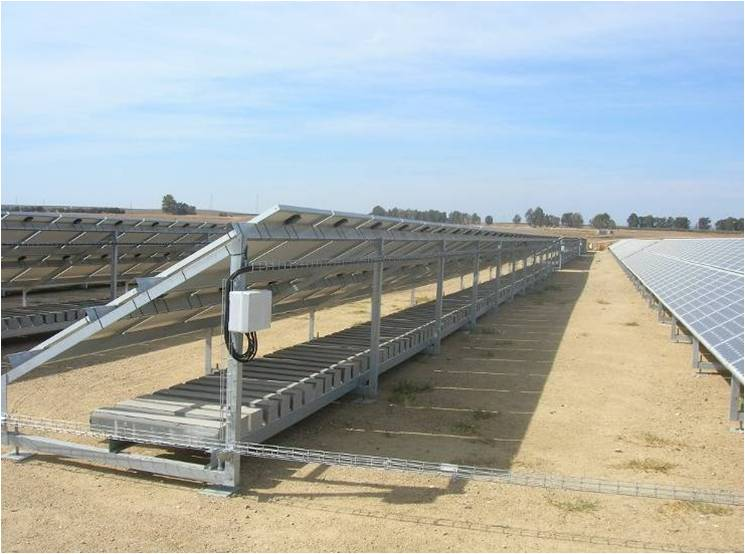
\includegraphics[scale=0.35]{../Fotos/EstructuraEstaticaSuelo}
\par\end{center}


\end{frame}

\begin{frame}
\frametitle{SFCR sobre suelo: seguimiento}
\begin{itemize}
\item \textbf{Fundamento:}

\begin{itemize}
\item Radiación incidente aumenta al seguir al sol
\item Pérdidas por reflexión disminuyen si el apuntamiento al sol mejora
\end{itemize}
\item Las diferentes técnicas de seguimiento son un \textbf{compromiso}
entre un \textbf{apuntamiento perfecto} y \textbf{sistemas estructurales
más económicos} y mejores \textbf{aprovechamientos del terreno}. 
\end{itemize}

\end{frame}

\begin{frame}
\frametitle{SFCR sobre suelo: seguimiento}
\begin{itemize}
\item \textbf{Doble eje}

\begin{itemize}
\item Apuntamiento {}``perfecto''
\item Mejor productividad, peor ocupación de terreno. 
\end{itemize}
\item \textbf{Seguimiento acimutal}

\begin{itemize}
\item Sacrifica un movimiento (inclinación del generador) para conseguir
sistemas más económicos. 
\end{itemize}
\item \textbf{Seguimiento horizontal con eje Norte-Sur}

\begin{itemize}
\item Sencillez y estabilidad estructural (el eje es horizontal y paralelo
al terreno, con tantos puntos de apoyo como se consideren necesarios), 
\item Facilidad de motorización, 
\item Buen aprovechamiento del terreno.
\end{itemize}
\end{itemize}

\end{frame}

\begin{frame}[plain]
\frametitle{Seguidor de eje horizontal N-S}

\begin{center}
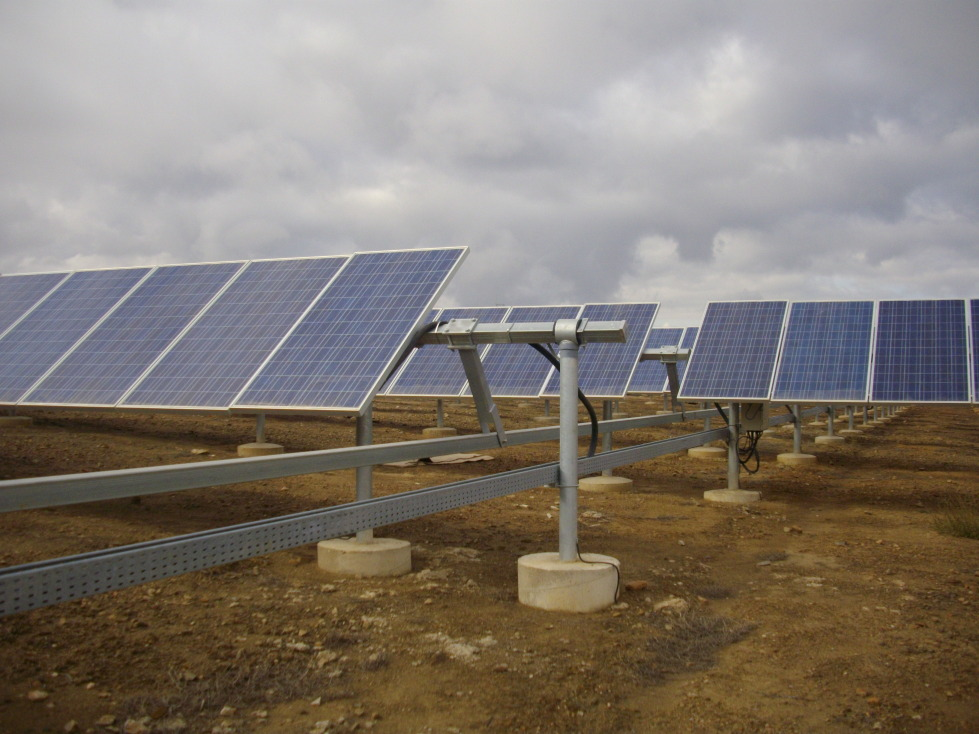
\includegraphics[scale=0.25]{../Fotos/SeguidorEjeHorizontal}
\par\end{center}


\end{frame}

\begin{frame}[plain]
\frametitle{Seguidor de doble eje}

\begin{center}
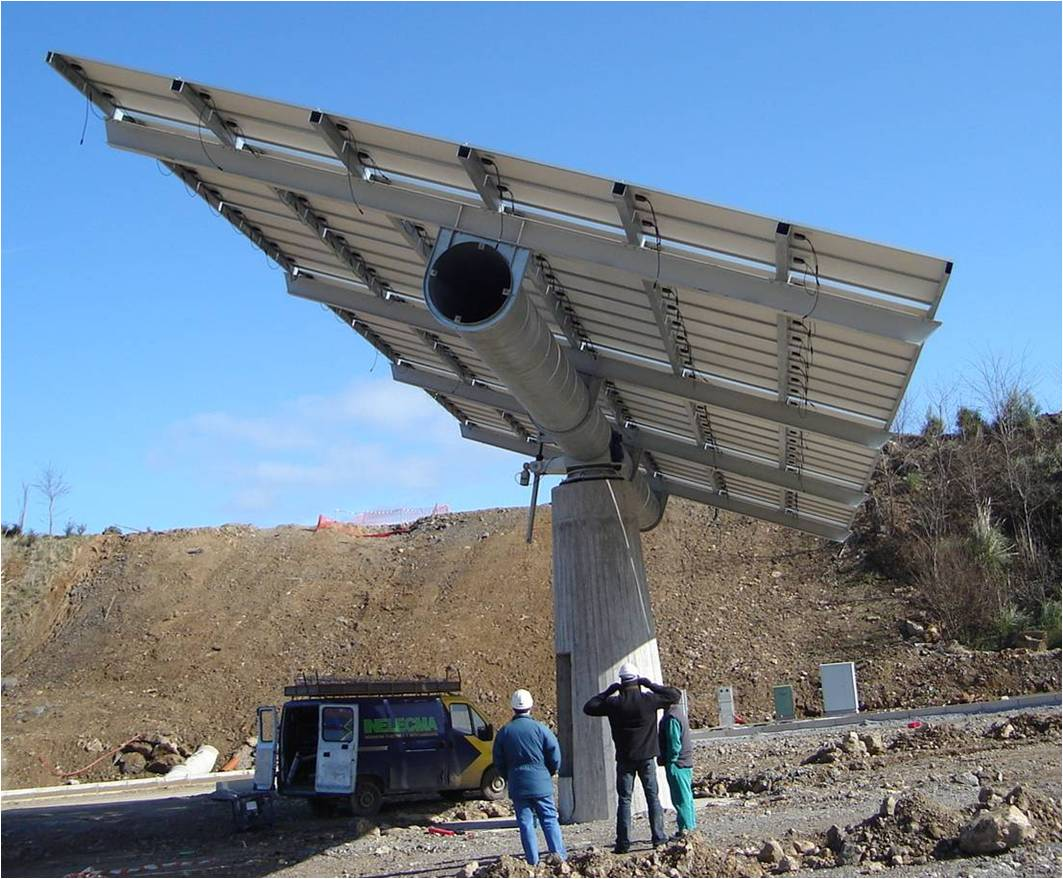
\includegraphics[scale=0.4]{../Fotos/SeguidorReocin}
\par\end{center}


\end{frame}

\section{Energía Producida por un SFCR}


\subsection{Procedimiento de cálculo}


\begin{frame}
\frametitle{Energía producida}

\[
E_{ac}=P_{g}^{*}\cdot\frac{G_{ef}}{G_{stc}}\cdot PR\cdot (1-FS)\]

\begin{itemize}
\item $E_{ac}$ es la \textbf{energía producida }en un periodo (\kWh)
\item $G_{stc}$ es la \textbf{irradiancia} en condiciones estándar de medida
(STC, $G_{stc}=\SI{1}{\kilo\watt\per\meter\squared}$, $T_c=\SI{25}{\celsius}$)
\item $P_{g}^{*}$ es la \textbf{potencia nominal} del generador FV ($\si{\kilo\wattpeak}$)
en STC
\item $G_{ef}$ es la \textbf{irradiación efectiva incidente} en el plano
del generador (\si{\kWh\per\meter\squared}) 
\item $PR$ es el \textbf{rendimiento del sistema} o \emph{performance ratio}
\item $FS$ es el \textbf{factor de sombras}
\end{itemize}

\end{frame}

\begin{frame}
\frametitle{Productividad}
\begin{block}
{}

En algunas ocasiones se habla de \textbf{productividad} del sistema,
$Y_{f}$, que es el cociente entre energía producida y potencia nominal
del sistema: \[
Y_{f}=\frac{E_{ac}}{P_{g}^{*}}\ (\si{\kilo\watthour\per\kilo\wattpeak})\]


\end{block}

\end{frame}

\begin{frame}
\frametitle{Performance Ratio}
\begin{block}
{Desglose de pérdidas}
\begin{itemize}
\item \textbf{Dispersión de parámetros} entre los módulos que componen el
generador (2-4\%)
\item \textbf{Tolerancia de potencia} de los módulos respecto a sus características
nominales (3\%)
\item \textbf{Temperatura} de funcionamiento de los módulos (5-8\%)
\item Conversión DC/AC realizada por el \textbf{inversor} (8-12\%)
\item \textbf{Efecto Joule} en los cables (2-3\%)
\item Conversión BT/MT realizada por el \textbf{transformador} (2-3\%)
\item \textbf{Disponibilidad} del sistema (0,5-1\%)
\end{itemize}
\end{block}

\end{frame}

\begin{frame}
\frametitle{Performance Ratio}
\begin{block}
{Valores reales}
\begin{itemize}
\item El análisis de funcionamiento de diversos sistemas FV europeos ha
mostrado que el rango de valores que toma el \emph{performance ratio}
es bastante amplio, con mínimos de 0,4 y máximos de 0,85. 
\item Para sistemas instalados desde 1996, \textbf{el valor promedio ha
sido de 0,74}. 
\end{itemize}
\end{block}

\end{frame}

\begin{frame}
\frametitle{Factor de sombras}
\begin{itemize}
\item \textbf{El factor de sombras suele tomar valores alrededor del 2 al
4\%}, tanto en instalaciones estáticas como de seguimiento. 
\item En casos específicos este factor puede ser más alto (por ejemplo,
debido a la existencia de edificios cercanos, o en aquellas plantas
con un nivel de ocupación de terreno superior al óptimo).
\end{itemize}

\end{frame}

\subsection{Radiación Efectiva según tipologías}

\begin{frame}[plain]
  \frametitle{Radiación en Sistema estático}

  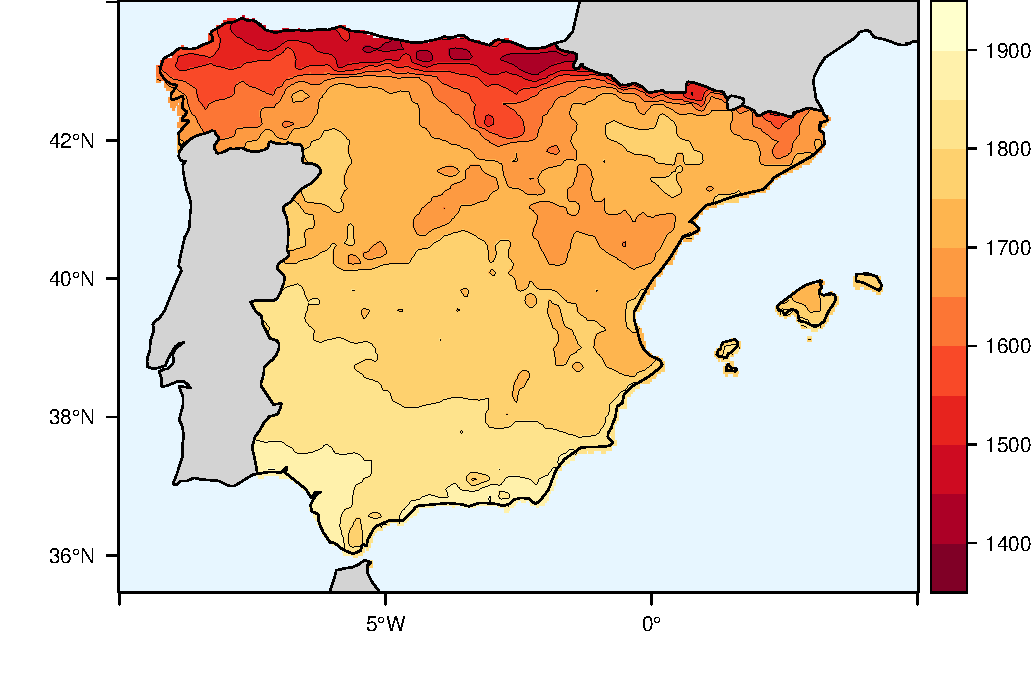
\includegraphics[width=\textwidth]{../Figuras/FixedKrig}
\end{frame}

\begin{frame}[plain]
  \frametitle{Radiación en Seguimiento Eje Horizontal}

  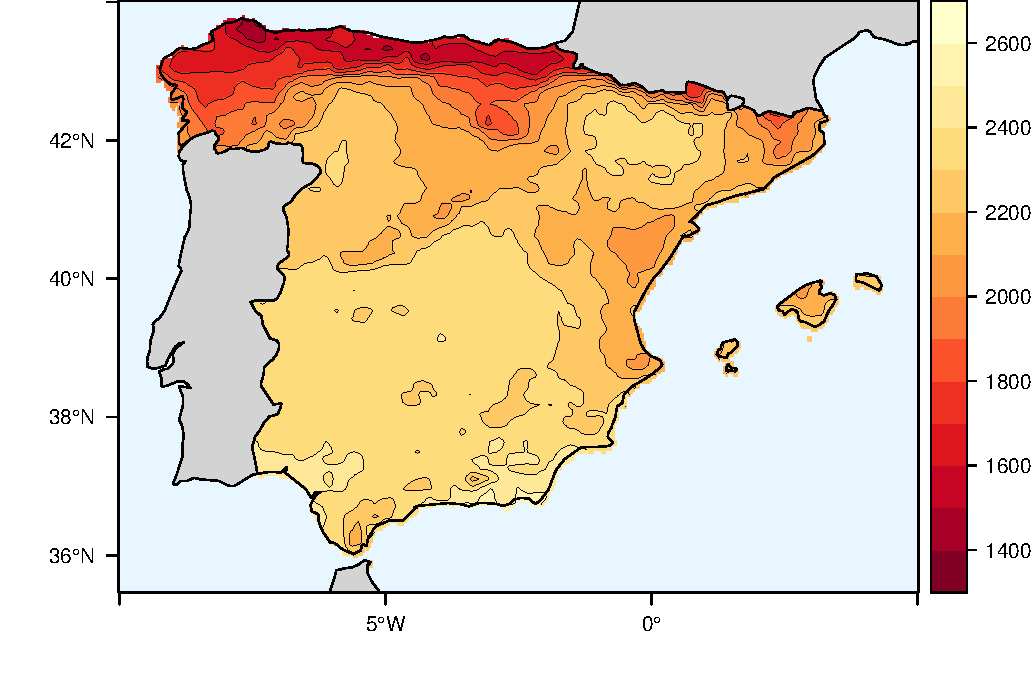
\includegraphics[width=\textwidth]{../Figuras/HorizKrig}

\end{frame}

\begin{frame}[plain]
  \frametitle{Radiación en Seguimiento Doble Eje}

  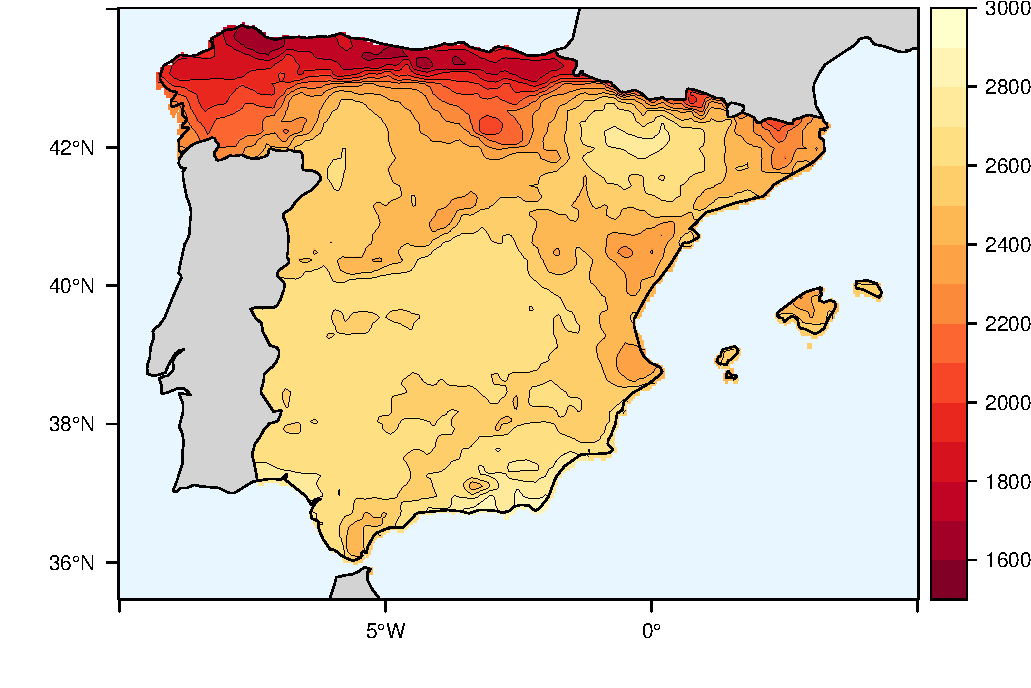
\includegraphics[width=\textwidth]{../Figuras/TwoKrig}

\end{frame}

\subsection{Comparación entre tipologías}

\begin{frame}[plain]
  \frametitle{Comparación Doble Eje-Estática}

  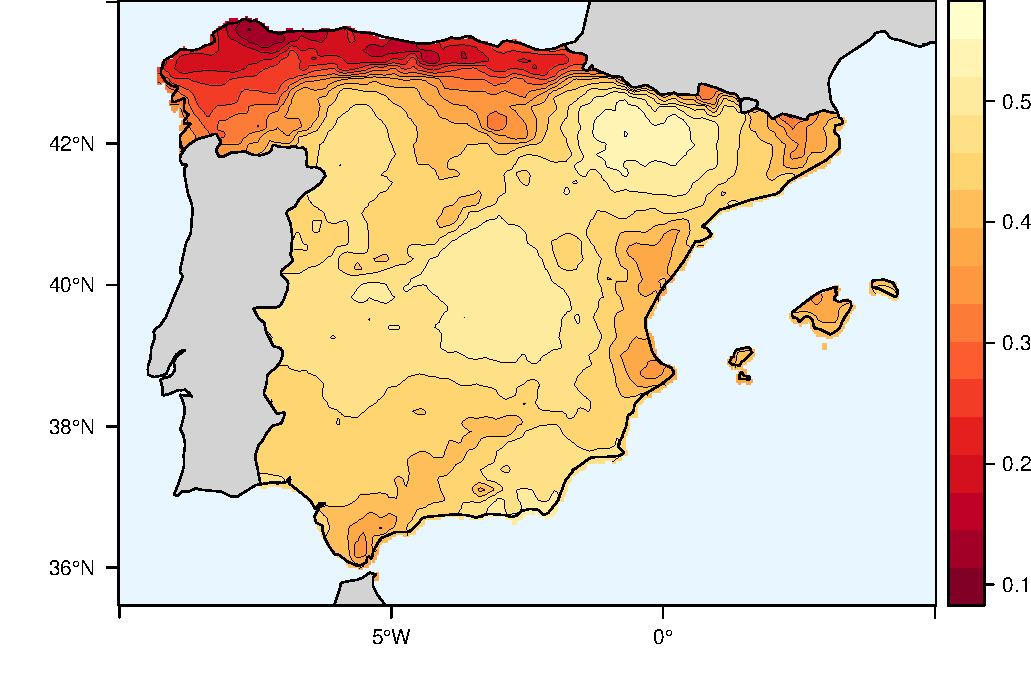
\includegraphics[width=\textwidth]{../Figuras/TwoFixed}


\end{frame}

\begin{frame}[plain]
  \frametitle{Comparación Doble Eje - Horizontal}

    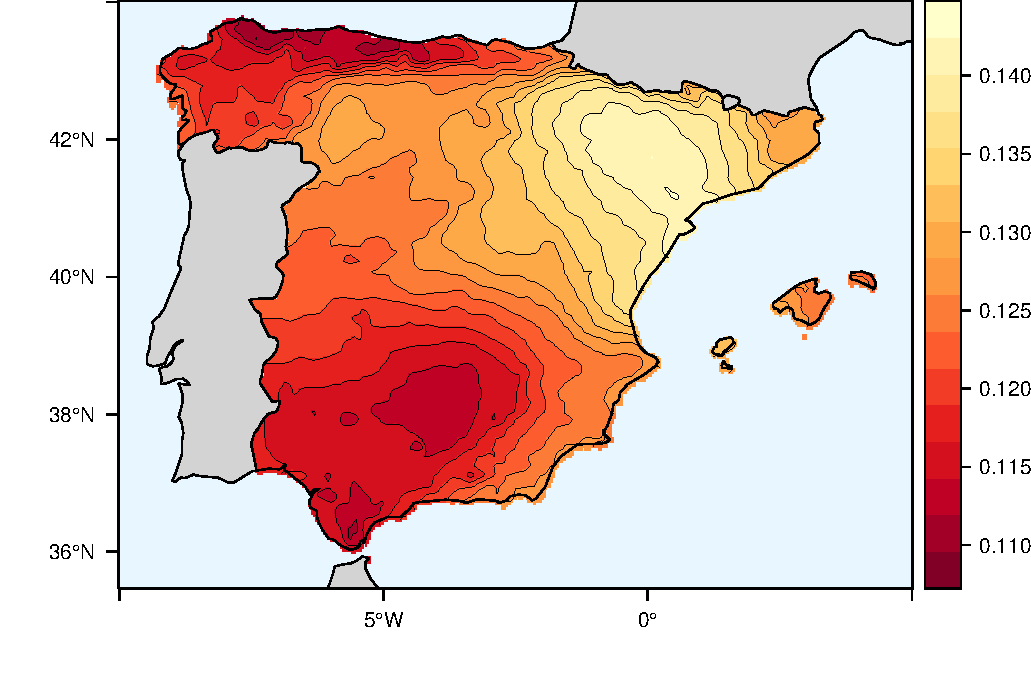
\includegraphics[width=\textwidth]{../Figuras/TwoHoriz}

\end{frame}

\begin{frame}[plain]
  \frametitle{Comparación Eje Horizontal - Estática}

    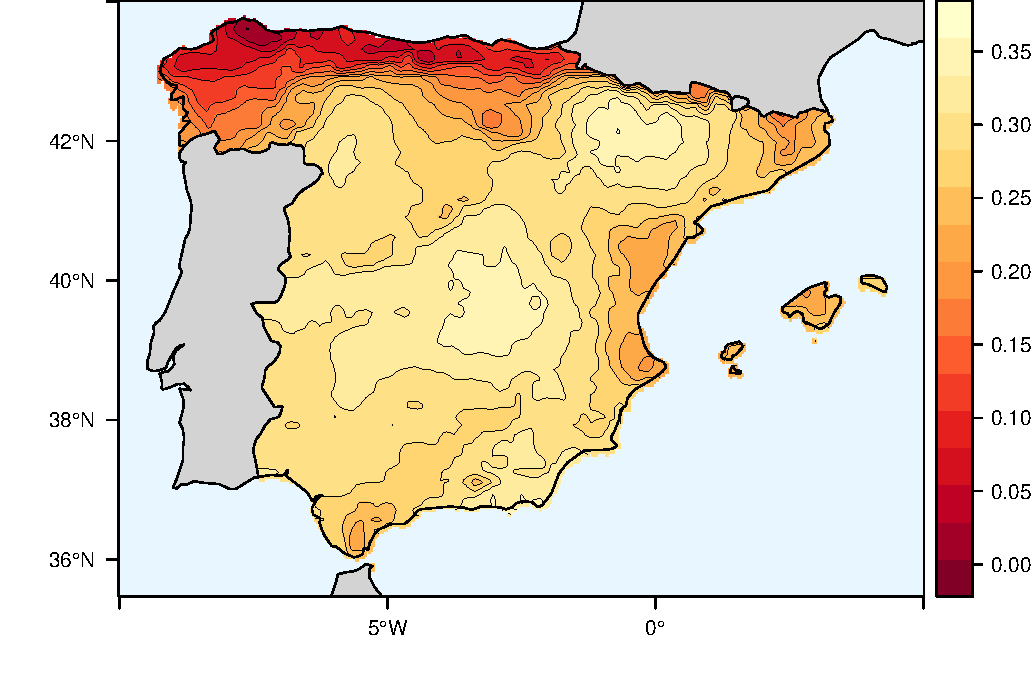
\includegraphics[width=\textwidth]{../Figuras/HorizFixed}

\end{frame}

\begin{frame}[plain]
  \frametitle{Comparación Eje Horizontal - Estática}
  \begin{columns}%{}


    \column{6cm}

    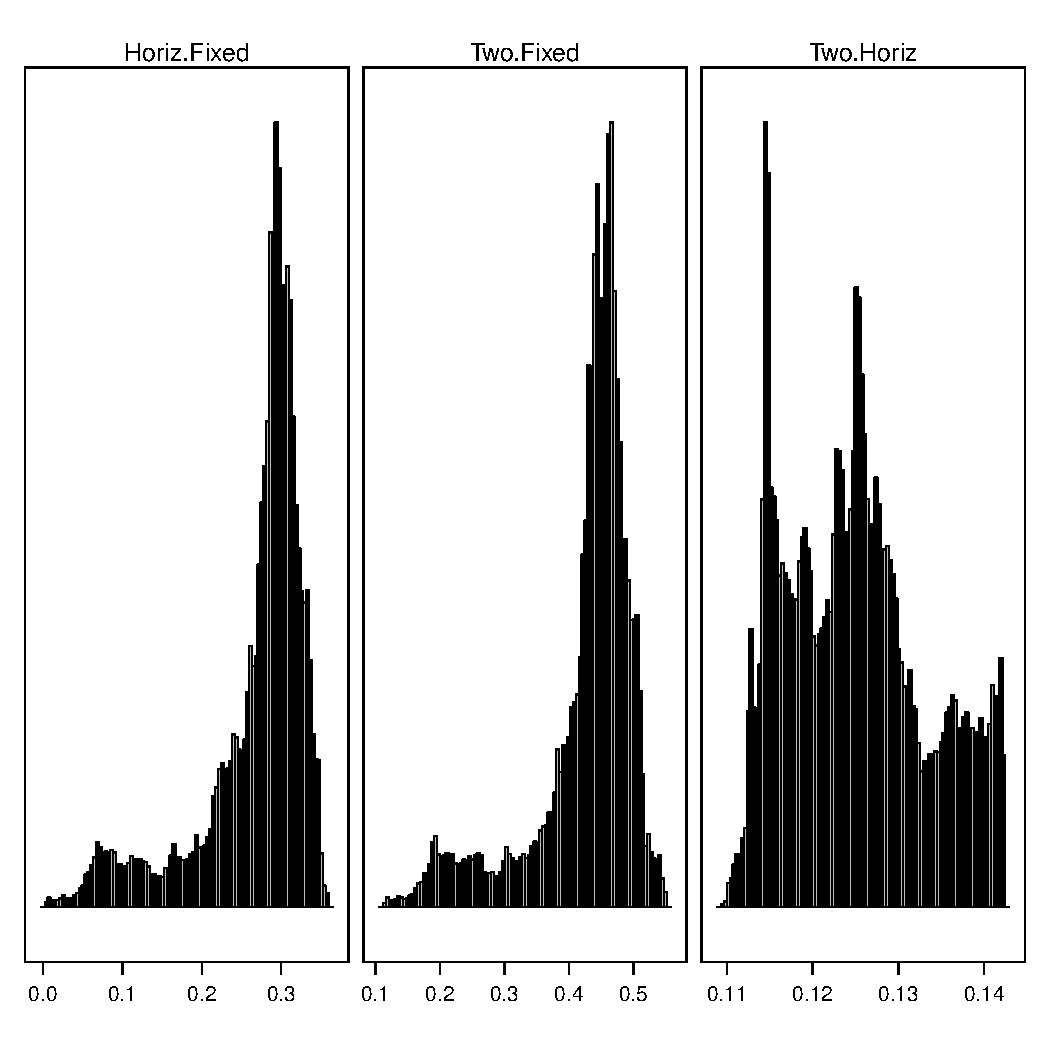
\includegraphics[width=6cm]{../Figuras/compSystems}

    \column{6cm}

    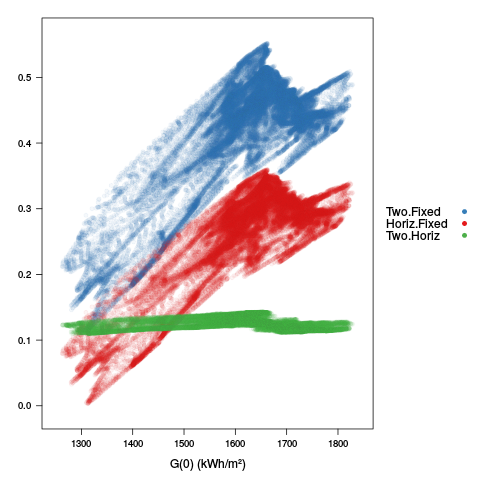
\includegraphics[width=6cm]{../Figuras/compSystemsG0}

  \end{columns}%{}
\end{frame}


\section{Tiempo de Retorno Energético}
\label{sec:epbt}

\begin{frame}
  \frametitle{Introducción}
  A lo largo de su ciclo de vida, además de producir energía y
  diferentes residuos, un sistema generador requerirá el empleo de
  energía para:
    \begin{itemize}
    \item Fabricación de componentes
    \item Tratamiento del terreno
    \item Transporte e instalación de los equipos
    \item Combustible necesario para su funcionamiento
    \item Reposición de equipos que agotan su ciclo
    \item ...
    \end{itemize}
\end{frame}

\begin{frame}
  \frametitle{Ciclo de Vida}

  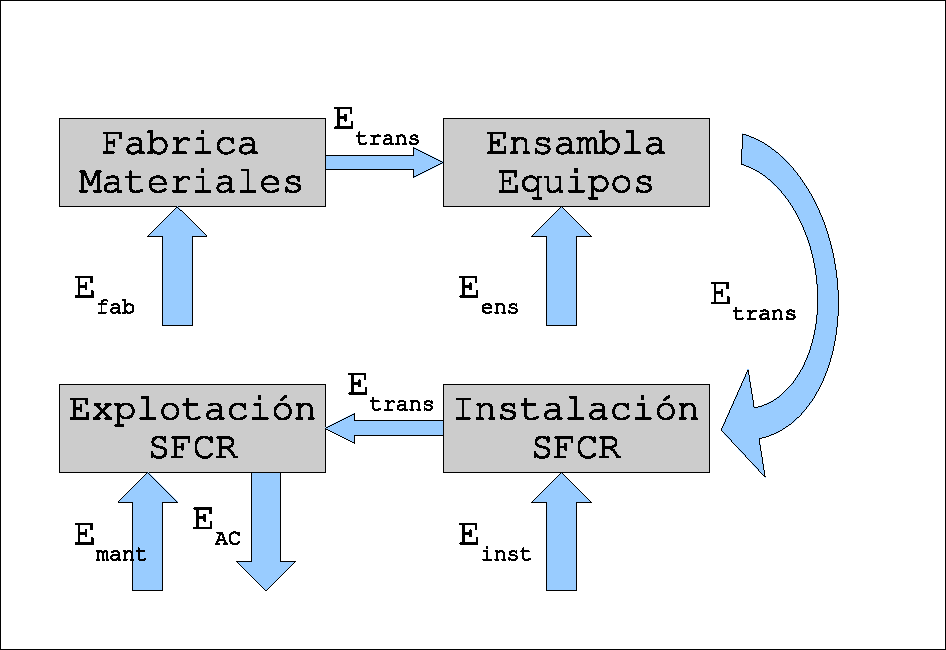
\includegraphics[width=\textwidth]{../Figuras/LCAFlujo}
  
\end{frame}

\begin{frame}
  \frametitle{Fuentes de Información}
    \begin{itemize}
    \item Inventarios de Ciclos de Vida (\emph{Life Cycle
        Inventory,} LCI) de los procesos empleados para
      implementar un SFCR. A partir de estos LCIs es posible
      estimar el impacto energético asociado.
      \begin{itemize}
      \item Incertidumbre alta en módulos FV (40\%)
      \end{itemize}
    \item Radiación global del lugar en el que el SFCR va a
      desempeñar sus funciones
    \item Características técnicas de los diferentes componentes
      del SFCR que permitan estimar la energía producida a lo
      largo de toda su vida útil.
    \end{itemize}
 
\end{frame}


\begin{frame}
  \frametitle{Energy PayBack Time}
  \begin{columns}
    \begin{column}{7cm}
          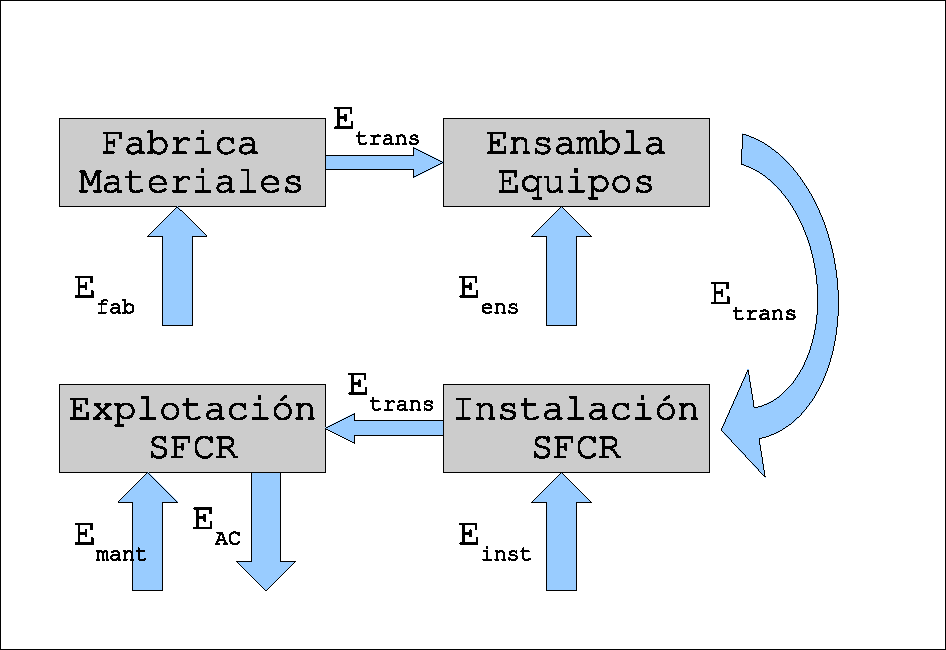
\includegraphics[width=\textwidth]{../Figuras/LCAFlujo}
    \end{column}
    \begin{column}{3cm}
      \begin{equation*}
        EPBT=\frac{E_{LCA}}{E_{ac}}
      \end{equation*}
    \end{column}
  \end{columns}
\end{frame}

\begin{frame}
  \frametitle{La cuestión del mix energético}
  \begin{itemize}
  \item La energía primaria depende de la eficiencia de conversión del
    sistema energético.
    \begin{itemize}
    \item Composición de fuentes energéticas (mix)
    \item Eficiencia para zona UCTE: 0.31
    \end{itemize}
  \item Proceso productivo de módulo FV es principalmente eléctrico
    (80\% de energía primaria se emplea en electricidad).
    \begin{itemize}
    \item Centros de fabricación en zonas con alta eficiencia de
      conversión.
    \item Menor impacto ambiental con alta penetración de renovables.
    \end{itemize}
  \item Un SFCR produce energía eléctrica normalmente distante de
    centro de fabricación: diferente eficiencia de conversión. 
    \begin{itemize}
    \item Menor EPBT inyectando en sistemas poco eficientes.
    \end{itemize}
  \end{itemize}

\end{frame}


\begin{frame}
  \frametitle{Energía de los principales componentes}
  \framesubtitle{Seguimiento a Doble Eje}
  \begin{tabular}{lll}
    \toprule
    Componente              &  ($MJ_{p}/kWp$)  &  (\%)     \\
    \midrule
    Módulo & 41\,819 & 69,54\% \\
    Estructura Soporte      &  9\,329          &  15,51\%  \\
    Mecanismos de seguimiento    &  248             &  0,41\%   \\
    Cimientos (acero)     &  3\,371          &  5,61\%   \\
    Cimientos (hormigón)  &  2\,445          &  4,07\%   \\
    Transporte              &  1\,339          &  2,23\%   \\
    Inversor               &  1,091           &  1,81\%   \\
    Cableado                 &  497             &  0,83\%   \\
    \midrule
    Total                  &  60\,140         &  100\%    \\
    \bottomrule
  \end{tabular}

\end{frame}

\begin{frame}
  \frametitle{Energía de los principales componentes}
  \framesubtitle{Seguimiento de Eje Horizontal NS}
  \begin{tabular}{lll}
    \toprule
    Componente              &  ($MJ_{p}/kWp$)  &  (\%)     \\
    \midrule
    Módulo & 41\,819 & 78,67\% \\
    Estructura Soporte      &  6\,108          &  11,49\%  \\
    Mecanismos de seguimiento    &  58              &  0,11\%   \\
    Cimientos (acero)     &  1\,536          &  2,89\%   \\
    Cimientos (hormigón)  &  1\,281          &  2,41\%   \\
    Transporte              &  900             &  1,69\%   \\
    Inversor               &  1\,091          &  2,05\%   \\
    Cableado                 &  364             &  0,68\%   \\
    \midrule
    Total                  &  53\,157         &  100\%    \\
    \bottomrule
  \end{tabular}
\end{frame}

\begin{frame}
  \frametitle{Energía de los principales componentes}
  \framesubtitle{Sistemas Estáticos}
  \begin{tabular}{lll}
    \toprule
    Componente              &  ($MJ_{p}/kWp$)  &  (\%)    \\
    \midrule
    Módulo & 41\,819 & 81,99\% \\
    Estructura Soporte      &  4\,459          &  8,74\%  \\
    Mecanismos de seguimiento    &  0               &  0,00\%  \\
    Cimientos (acero)     &  0               &  0,00\%  \\
    Cimientos (hormigón)  &  2\,352          &  4,61\%  \\
    Transporte              &  1\,037          &  2,03\%  \\
    Inversor               &  1\,091          &  2,14\%  \\
    Cableado                 &  248             &  0,49\%  \\
    \midrule
    Total                  &  51\,005         &  100\%   \\
    \bottomrule
  \end{tabular}
\end{frame}

\begin{frame}
  \frametitle{Valores de EPBT por sistema}
  \begin{tabular}{ccccccc}
    \toprule
    EPBT & 1st. Quartile & Median & Mean & 3rd Quartile \tabularnewline
    \midrule 
    Doble Eje & 2,4 & 2,6 & 2,7 & 2,82\tabularnewline
    Horizontal-NS &  2,65 & 2,88 & 3 & 3,17\tabularnewline
    Estático & 3 & 3,22 & 3,3 & 3,45\tabularnewline
    \bottomrule 
  \end{tabular}

\end{frame}

\begin{frame}
  \frametitle{Doble Eje}
  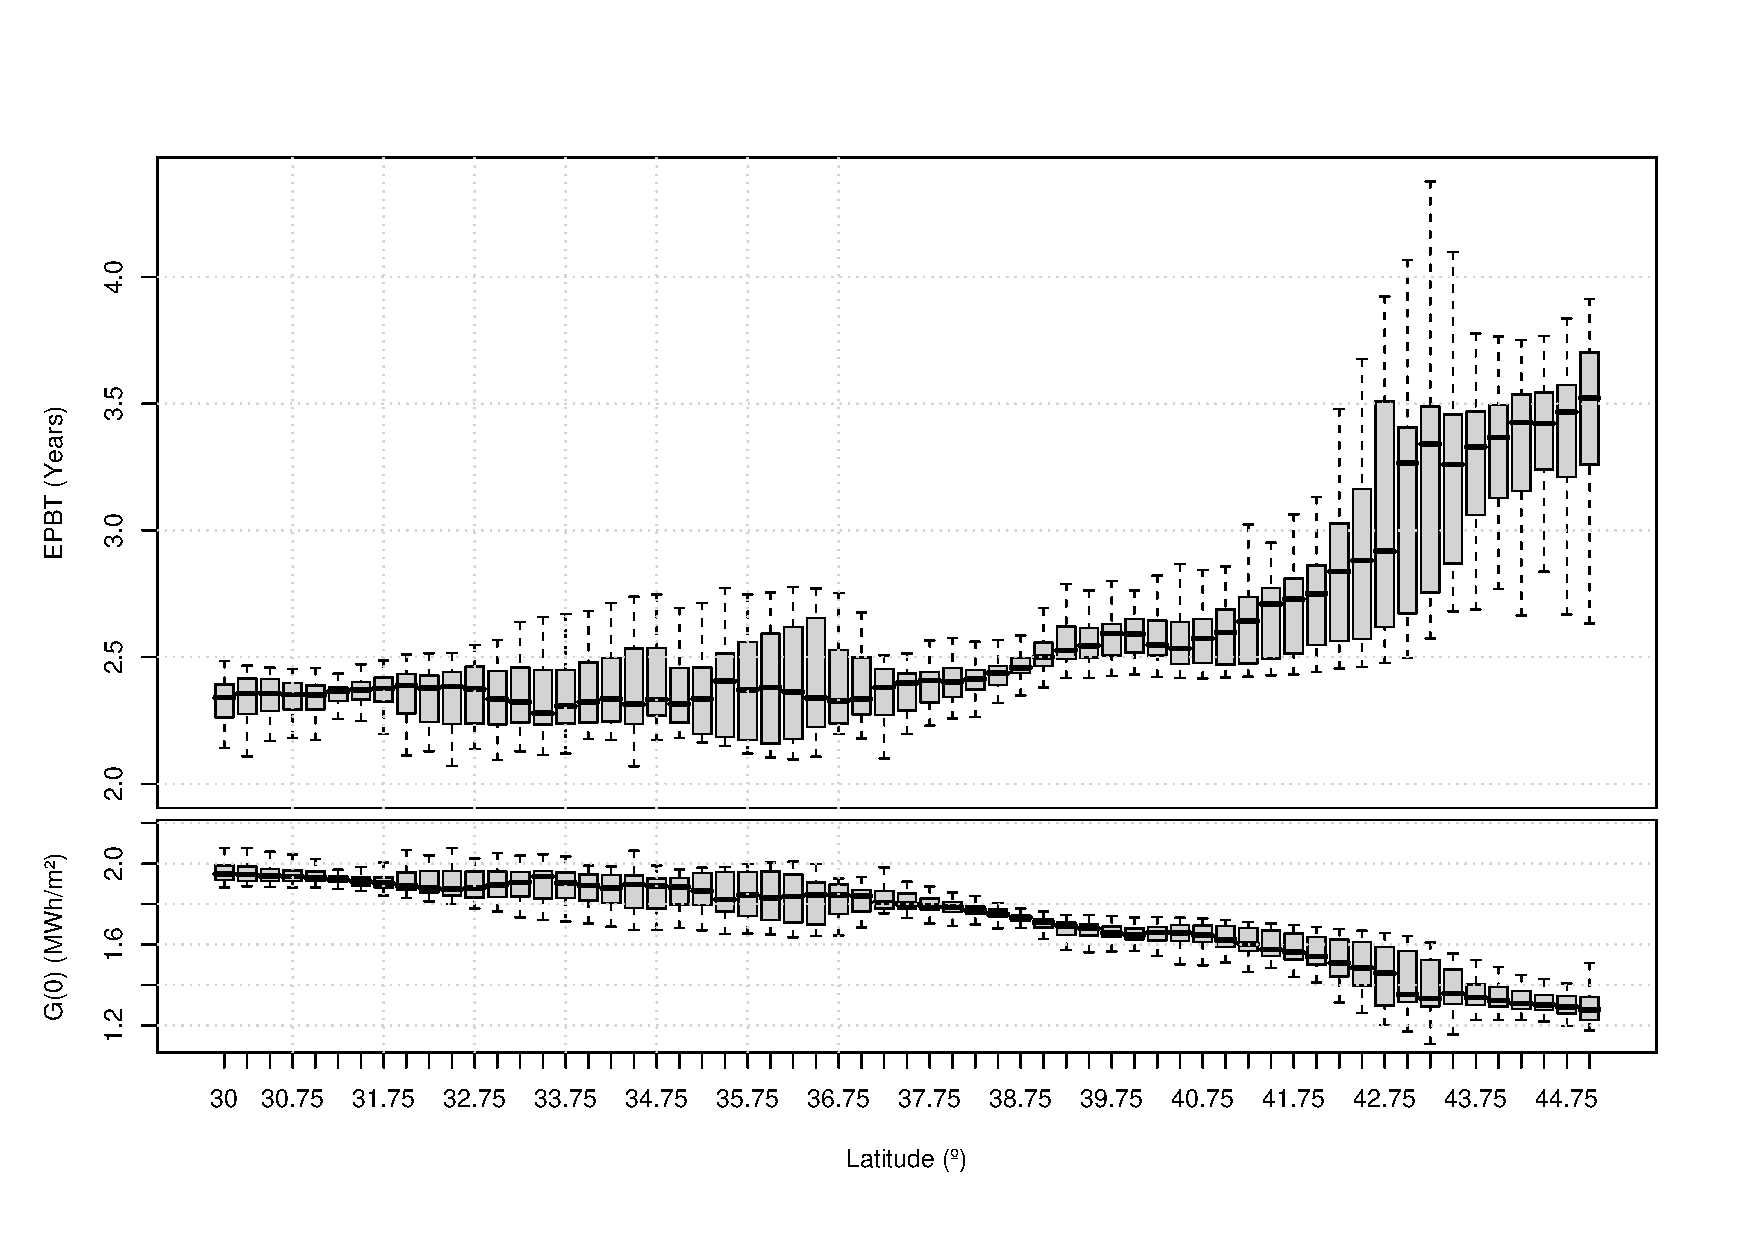
\includegraphics[width=\textwidth]{../Figuras/BoxPlotEPBTEuropa_2x}
\end{frame}

\begin{frame}
  \frametitle{Horizontal NS}
  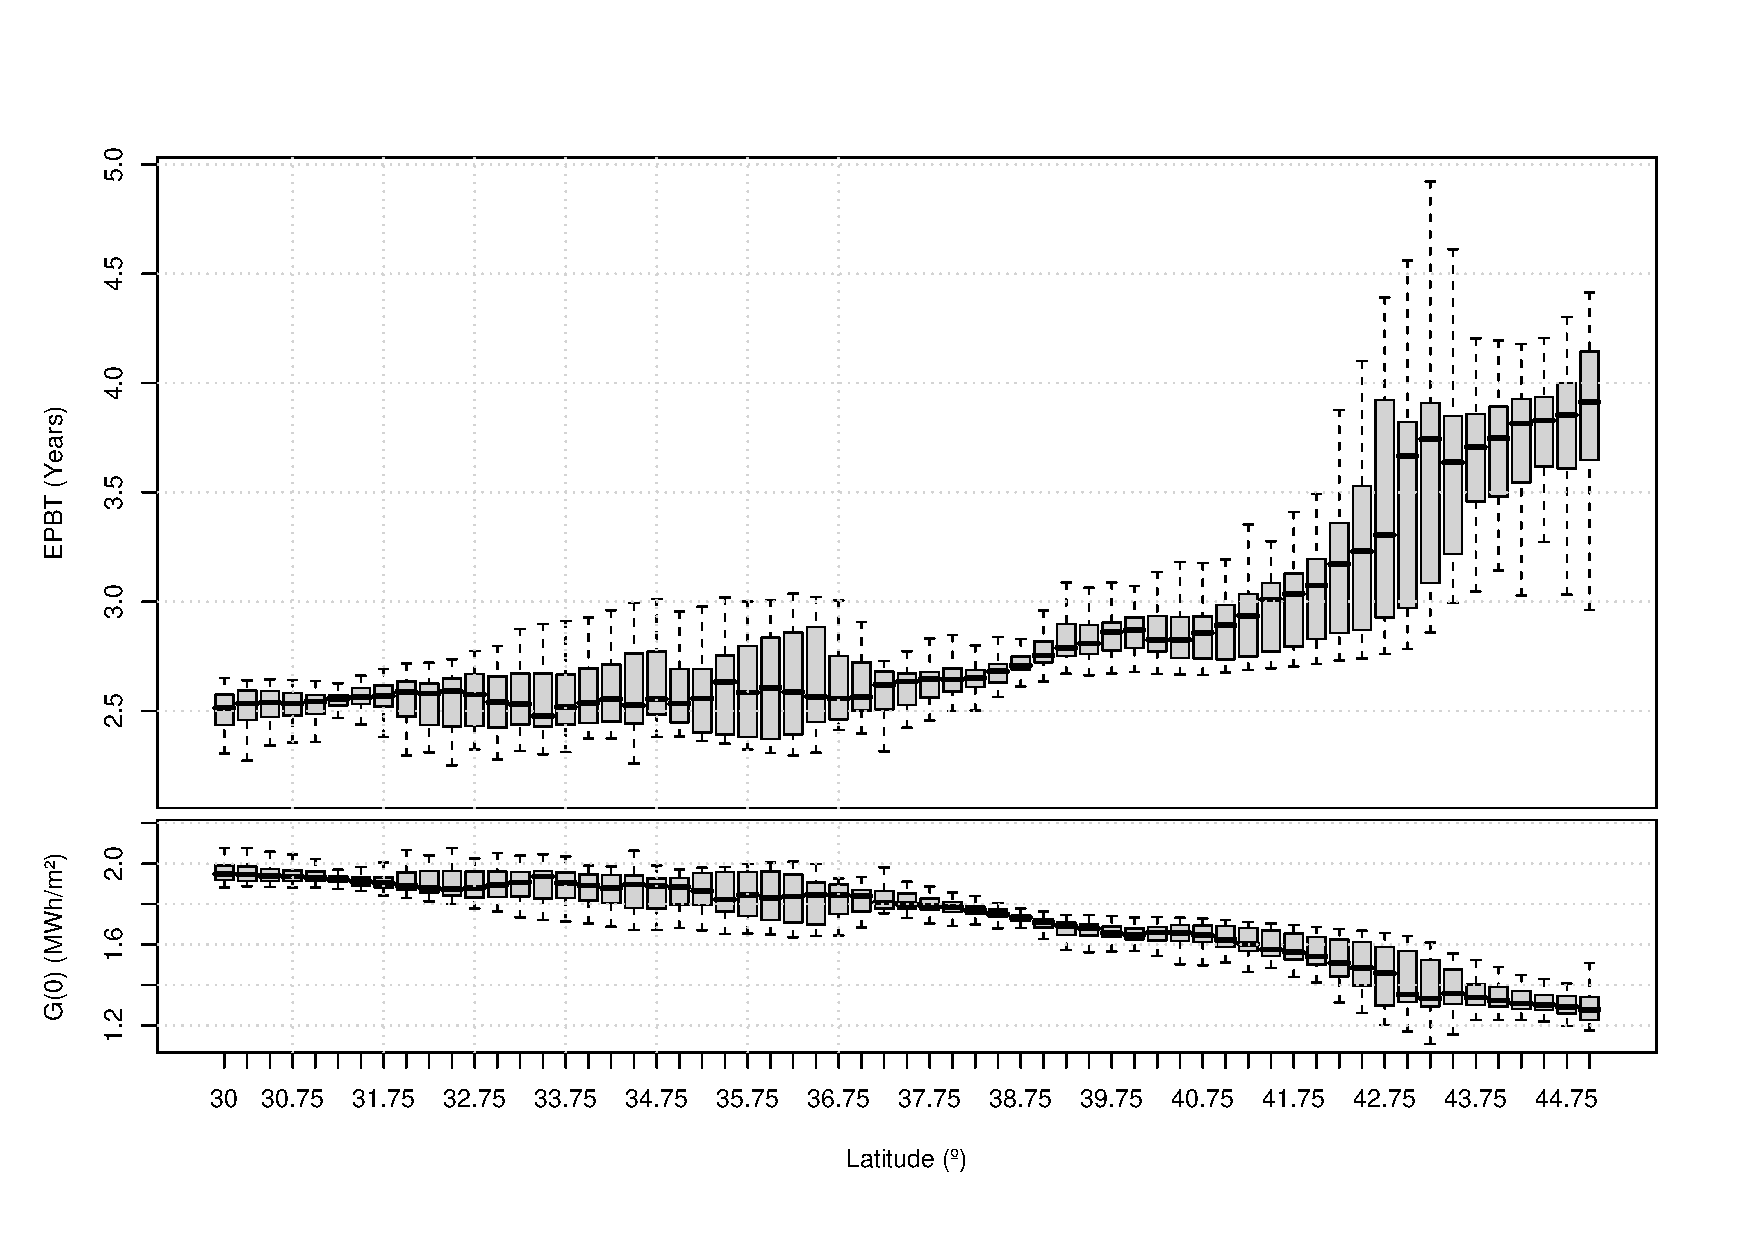
\includegraphics[width=\textwidth]{../Figuras/BoxPlotEPBTEuropa_HorizNS}
\end{frame}

\begin{frame}
  \frametitle{Estático}
  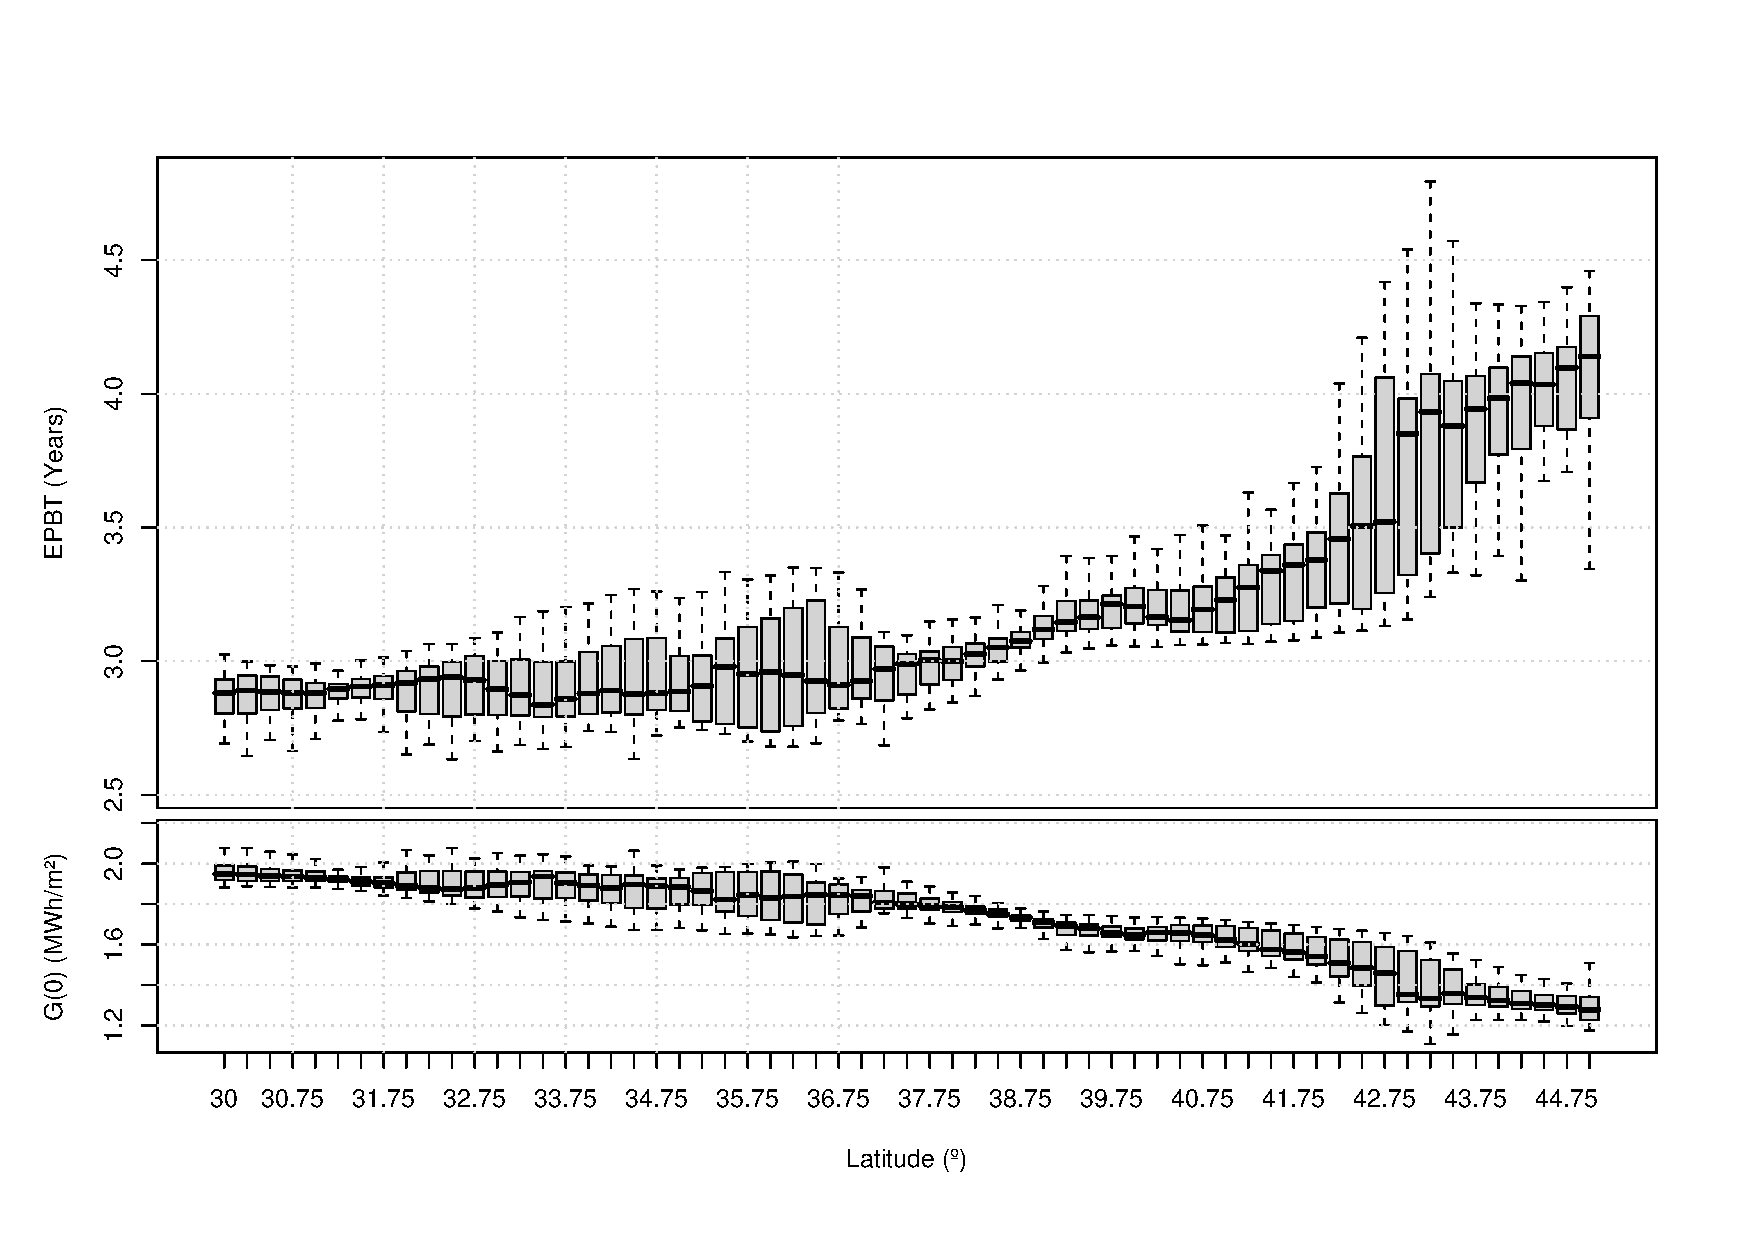
\includegraphics[width=\textwidth]{../Figuras/BoxPlotEPBTEuropa_Fixed}
\end{frame}

\begin{frame}
  \frametitle{Comparativa}
  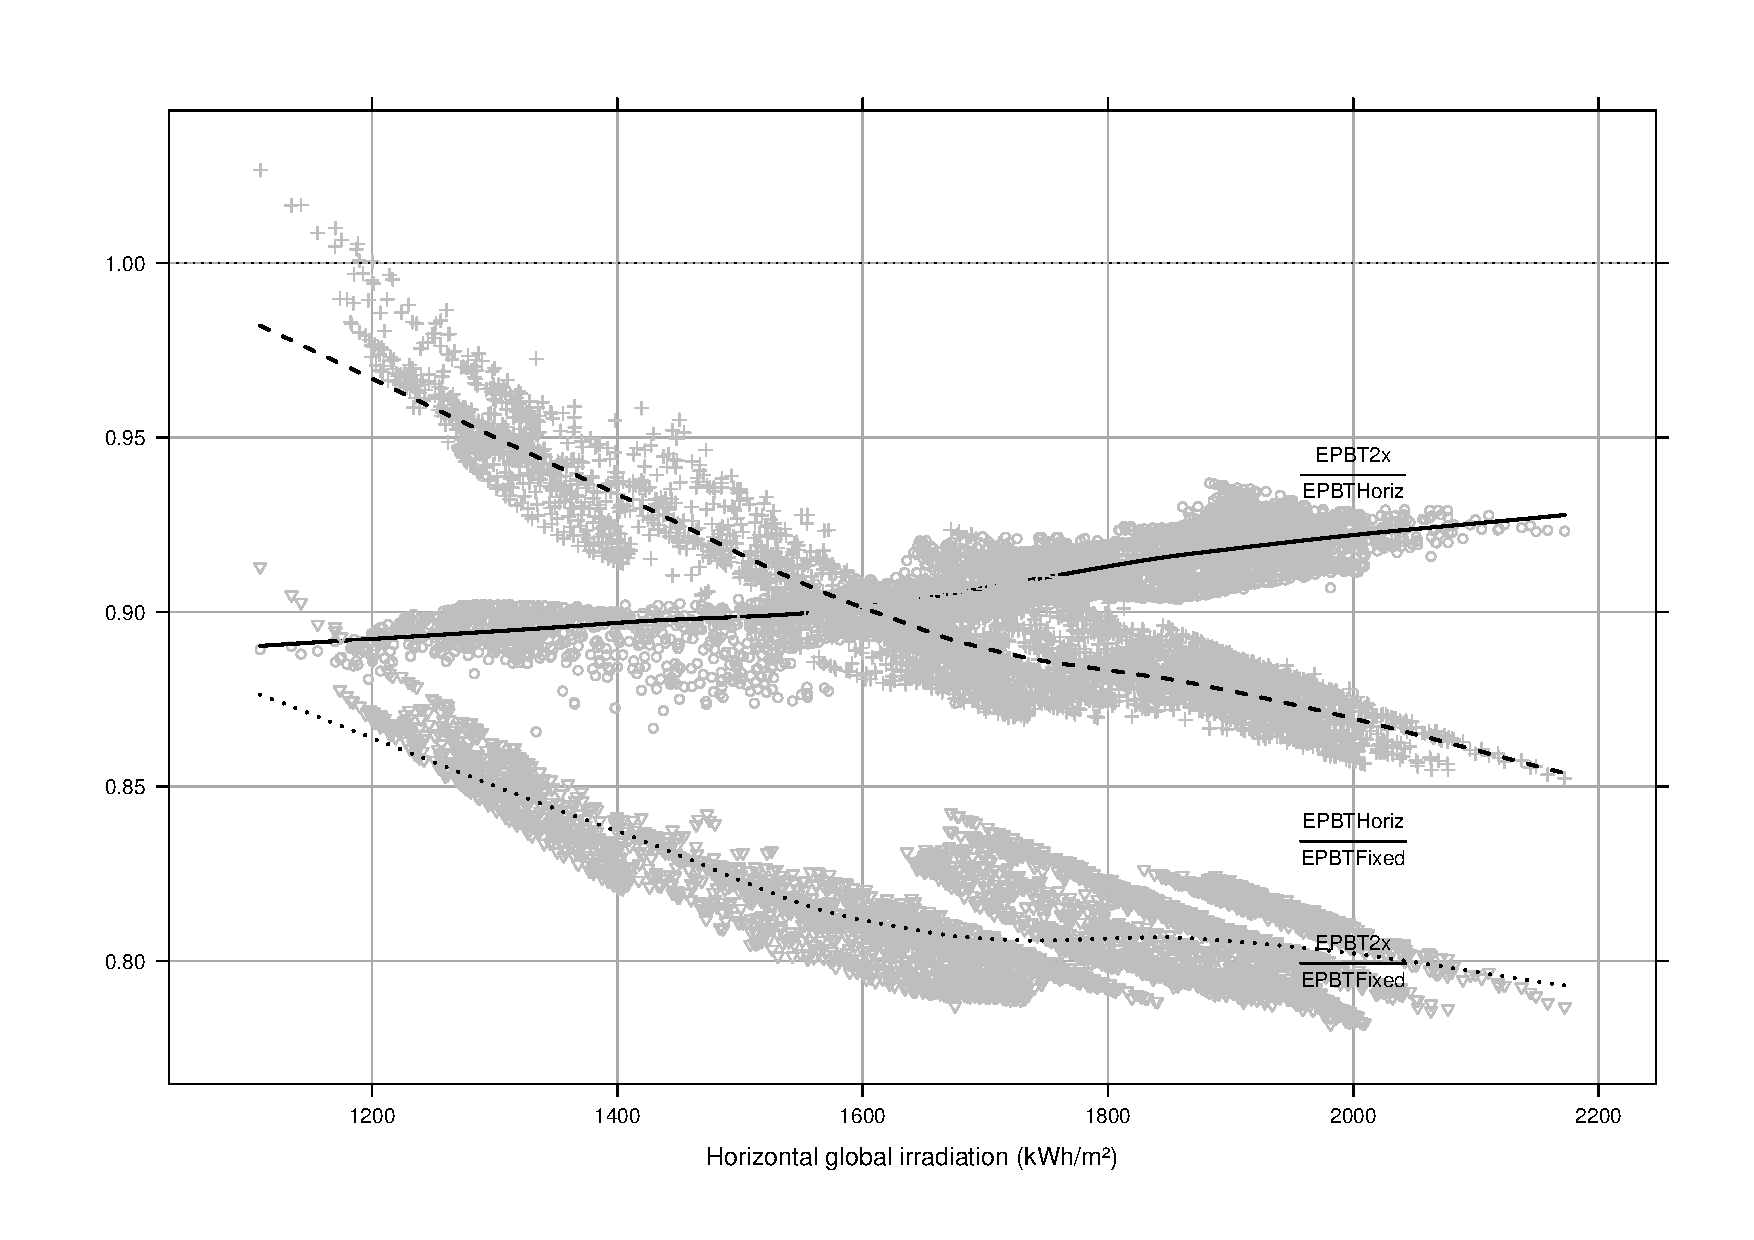
\includegraphics[width=\textwidth]{../Figuras/EPBTEuropavsGh2}
\end{frame}

\section{Configuración de sistemas}


\begin{frame}
\frametitle{Configuración del generador}

Para elegir una \textbf{configuración eléctrica} deben tenerse en
cuenta diferentes aspectos:
\begin{itemize}
\item Adecuación a la \textbf{ubicación física} de los módulos en la estructura.
\item La \textbf{curva de eficiencia del inversor} depende de la tensión
de entrada.
\item \textbf{Inversión y rendimiento económicos}.
\item \textbf{Espacio disponible}.
\item \textbf{Relación de potencias} de generador e inversor.
\end{itemize}

\end{frame}

\begin{frame}
\frametitle{Configuración eléctrica y estructura}
\begin{itemize}
\item Es recomendable elegir \textbf{series} compuestas por un número de
módulos que puedan ser ubicados en una \textbf{única hilera de la
estructura}. 

\begin{itemize}
\item \textbf{Se facilita el trazado del cableado}: la propia estructura
puede servir como fijación auxiliar, se evitan cruzamientos indeseados.
\item \textbf{Se minimiza la influencia de las sombras}: es muy frecuente
la aparición de sombras entre partes del generador o entre seguidores,
sombras de forma rectangular y que comienzan afectando a las partes
bajas de la estructura. Al cablear por hileras, las sombras de las
hileras bajas no afectan a las hileras inmediatamente superiores.
\end{itemize}
\end{itemize}

\end{frame}

\begin{frame}
\frametitle{Potencia del generador}
\begin{itemize}
\item La potencia del generador fotovoltaico está relacionada directamente
con la \textbf{inversión económica} a realizar. 
\item Por otra parte, la relación entre \textbf{energía generada} y potencia
nominal es aproximadamente lineal, y por tanto, los \textbf{ingresos
económicos} dependen casi linealmente de la potencia del generador. 
\item Por tanto, para decidir la potencia del generador ($P_{g}^{*}=N_{s}\cdot N_{p}\cdot P_{m}^{*}$)
debe tenerse en cuenta el capital o financiación disponible, y el
rendimiento económico deseado.
\end{itemize}

\end{frame}

\begin{frame}
\frametitle{Potencia del generador}
\begin{itemize}
\item La potencia del generador es proporcional al área del generador y
al \textbf{terreno ocupado }(que también influye, aunque en menor
grado, en el cálculo económico). Por tanto, debe tenerse en cuenta
el espacio disponible (o el coste que se pretende asumir por el uso
de terreno).
\item Según el \textbf{tipo de sistema} (estático, seguimiento) se debe
elegir una relación de potencias de generador e inversor.
\end{itemize}

\end{frame}

\subsection{Sistemas Estáticos}


\begin{frame}[plain]
\frametitle{Inclinación y Orientación}

\[
\beta_{opt}=3.7+0.69\cdot|\phi|\]


\begin{center}
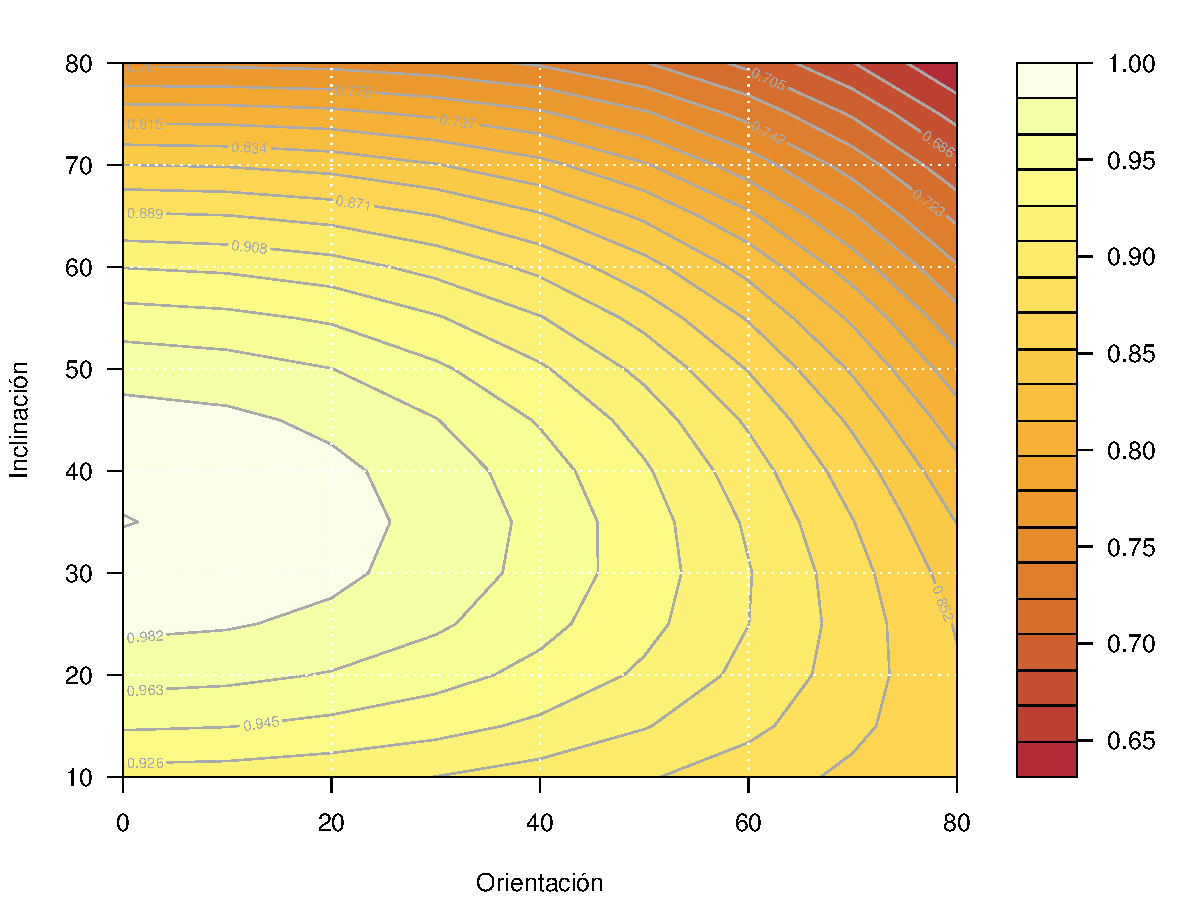
\includegraphics[scale=0.5]{../Figuras/PorcentajeProduccionEdificios}
\par\end{center}


\end{frame}

\begin{frame}
\frametitle{Pérdidas angulares según CTE}

\[
\mathrm{
  \begin{cases}
    100\cdot[1,2\cdot10^{-4}\cdot(\beta-\phi+10)^{2}+3,5\cdot10^{-5}\cdot\alpha^{2}]
    & 15\degree<\beta<90\degree\\
    100\cdot[1,2\cdot10^{-4}\cdot(\beta-\phi+10)^{2}] &
    \beta<15\degree
  \end{cases}}
\]

\begin{center}
\begin{tabular}{>{\centering}m{3cm}>{\centering}m{3cm}cc}
\toprule 
\textrm{Caso} & \textrm{Orientación e inclinación} & \textrm{Sombras} & \textrm{Total}\tabularnewline
\midrule
\midrule 
\textrm{General } & \textrm{10} & \textrm{10} & \textrm{15}\tabularnewline
\midrule 
\textrm{Superposición} & \textrm{20} & \textrm{15} & 30\tabularnewline
\midrule 
\textrm{Integración arquitectónica} & 40 & 20 & 50\tabularnewline
\bottomrule
\end{tabular}
\par\end{center}


\end{frame}

\begin{frame}
\frametitle{Sombras entre filas}

\begin{center}
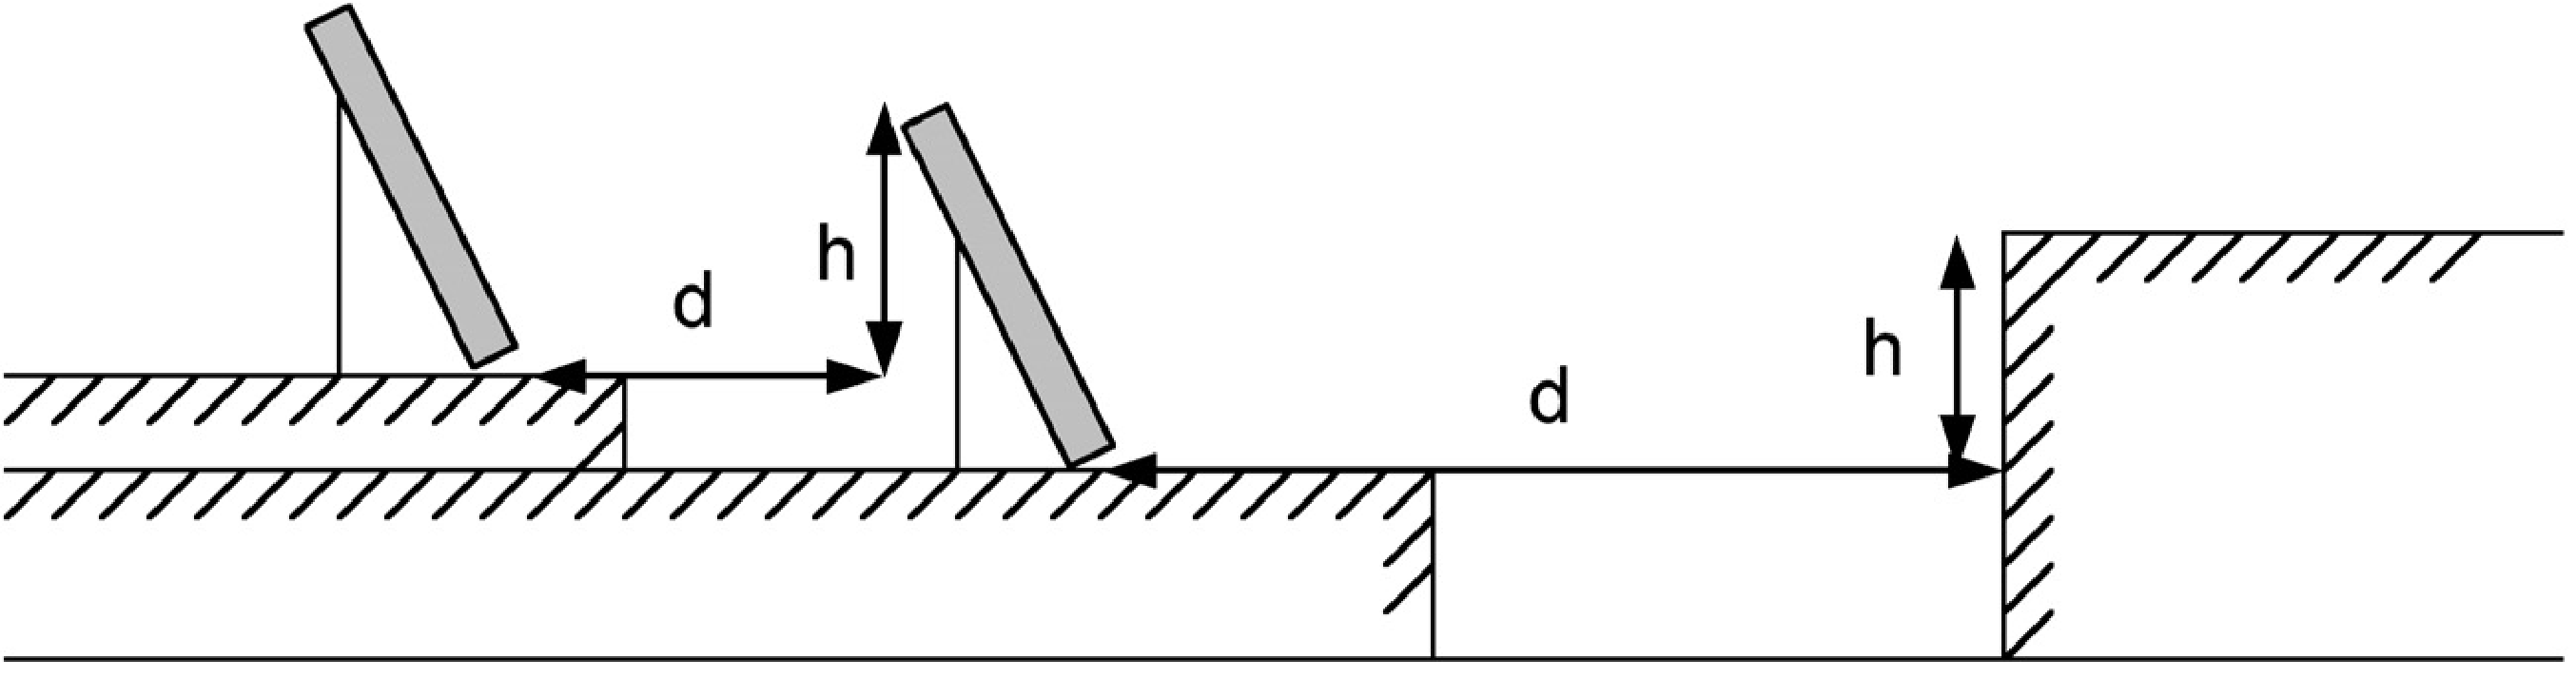
\includegraphics[clip,scale=0.25]{../Figuras/Figuras_Externas/SombraEstaticaInclinado2}
\par\end{center}


\end{frame}

\begin{frame}
\frametitle{Sombras entre filas}

Suele establecerse un objetivo de \textbf{4 horas de sol en torno
al mediodía del solsticio de invierno libres de sombra}. 

La longitud de la sombra de un obstáculo se mide con:\[
d=\frac{h}{\tan\gamma_{s}}\]


En el mediodía del solsticio de invierno \[
\gamma_{s}=90-23.45-\phi\simeq67-\phi\]
Para 2 horas antes y después:

\[
d_{min}=\frac{h}{\tan(61\degree-\phi)}\]



\end{frame}

\begin{frame}
\frametitle{Separación de Estructuras estáticas}
\begin{columns}%{}


\column{3cm}

\begin{center}
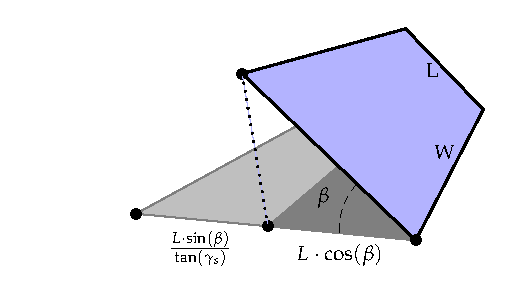
\includegraphics[scale=0.45]{../Figuras/DimensionesSeguidorSombra}
\par\end{center}

\[
W=\infty\]
\[
ROT=D/L\]



\column{7cm}

\begin{center}
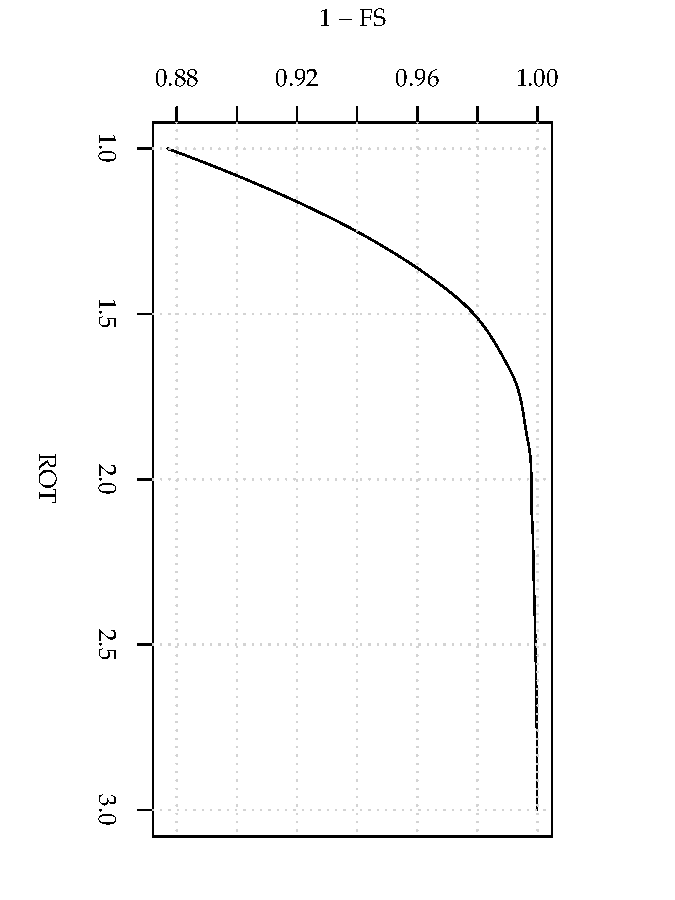
\includegraphics[scale=0.5, angle=90]{../Figuras/AbacoSombraEst_Ene10}
\par\end{center}

\end{columns}%{}

\end{frame}

\subsection{Seguidores de eje horizontal NS}


\begin{frame}
\frametitle{Separación de Seguidores Eje Horizontal}
\begin{columns}%{}


\column{5cm}

\begin{center}
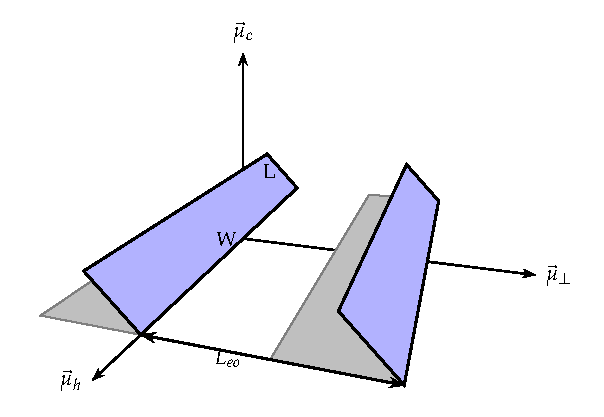
\includegraphics[scale=0.75]{../Figuras/SombrasHoriz}
\par\end{center}


\column{3cm}

\[
W=\infty\]
\[
ROT=L_{eo}/L\]


\end{columns}%{}

\end{frame}

\begin{frame}
\frametitle{Separación de Seguidores Horizontal N-S}


\framesubtitle{Sombra}

\begin{center}
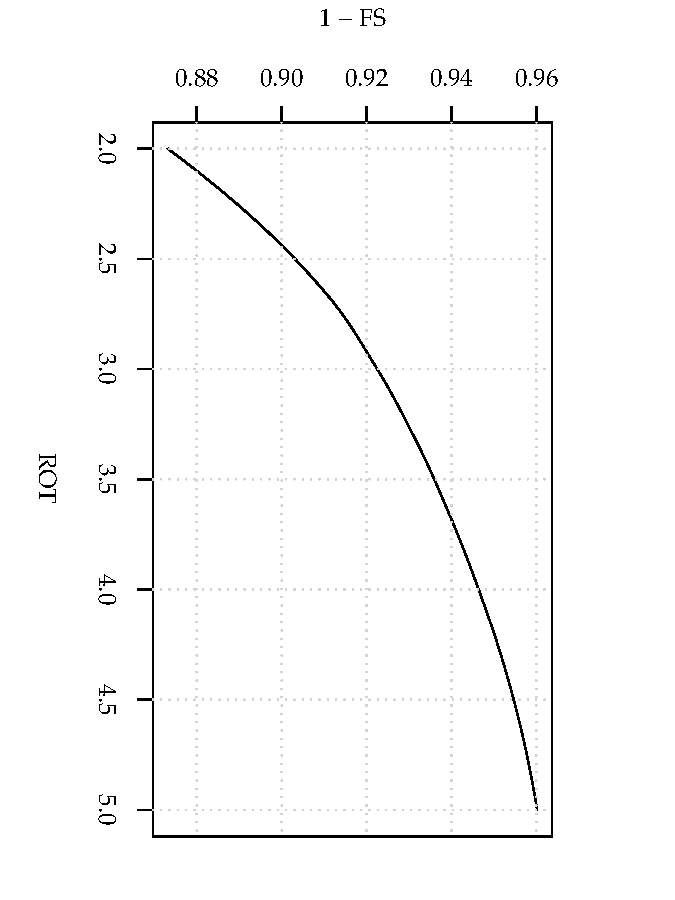
\includegraphics[scale=0.61, angle=90]{../Figuras/AbacoSeguidorHorizSombra_Ene10}
\par\end{center}


\end{frame}

\begin{frame}
\frametitle{Backtracking}
\begin{itemize}
\item El \textbf{sombreado} en un generador puede producir problemas por
el efecto de \textbf{punto caliente}.
\item En seguidores de eje horizontal se puede \textbf{evitar la incidencia
de sombras} en cualquier instante mediante el {}``\textbf{backtracking}'':

\begin{itemize}
\item Al \textbf{amanecer} el seguidor está en posición \textbf{horizontal}.
\item Según avanza el día el seguidor gira en \textbf{sentido contrario
al movimiento solar para evitar las sombras}.
\item En un determinado momento se cruza con el sol y puede continuar el
movimiento {}``convencional''.
\item En un instante de la tarde debe volver a cambiar el sentido hasta
la \textbf{horizontal en la noche}.
\end{itemize}
\end{itemize}

\end{frame}

\begin{frame}
\frametitle{Backtracking}

\begin{center}
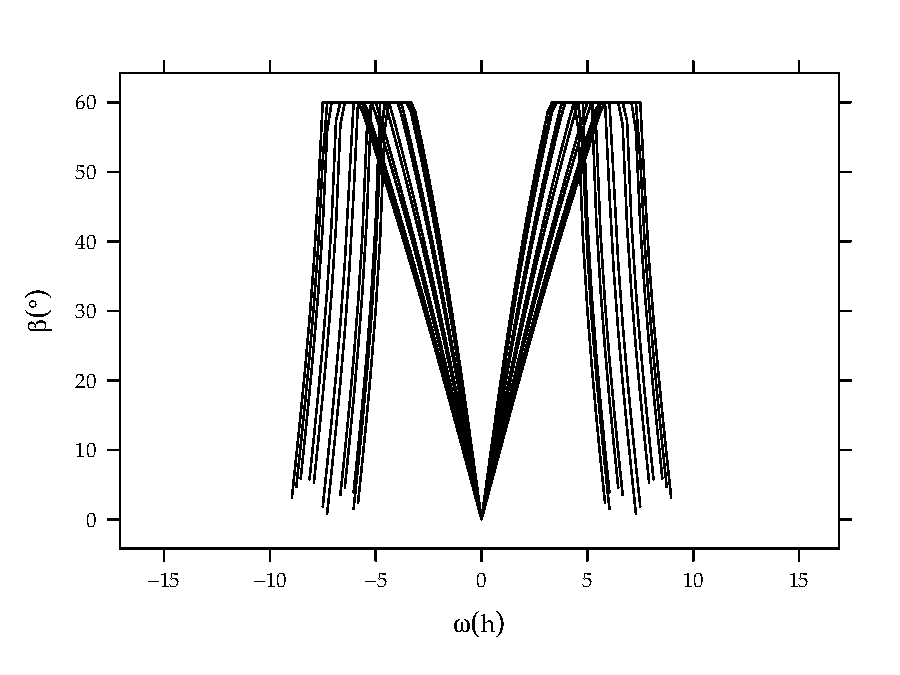
\includegraphics[scale=0.65]{../Figuras/BackTracking}
\par\end{center}


\end{frame}

\begin{frame}
\frametitle{Separación de Seguidores Horizontal N-S}


\framesubtitle{Backtracking}

\begin{center}
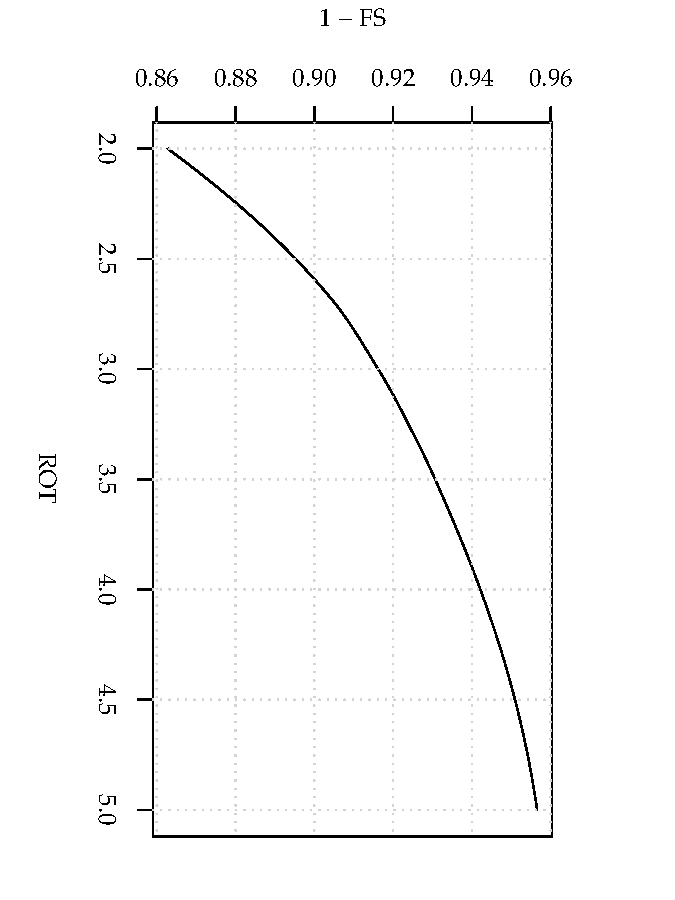
\includegraphics[scale=0.61, angle=90]{../Figuras/AbacoHorizBT_Ene10}
\par\end{center}


\end{frame}

\subsection{Seguidores doble eje}



\begin{frame}
\frametitle{Separación de seguidores Doble Eje}
\begin{columns}%{}


\column{7cm}

\begin{center}
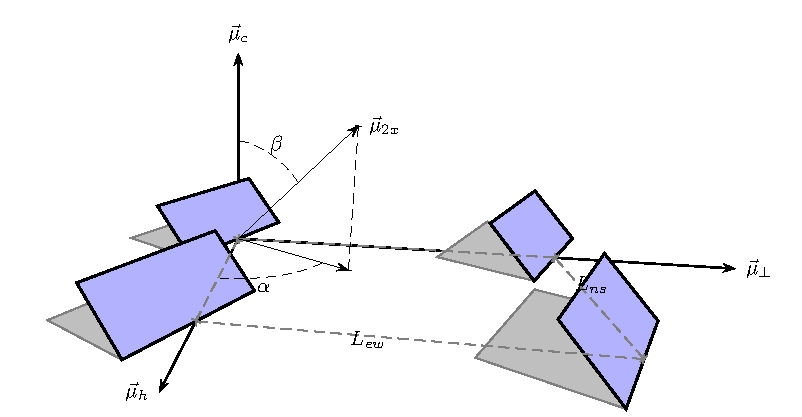
\includegraphics[scale=0.6]{../Figuras/Sombra2X} 
\par\end{center}


\column{3cm}

\begin{center}
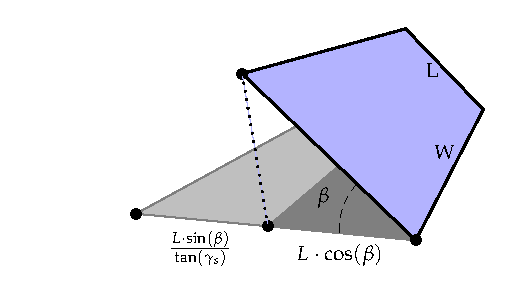
\includegraphics[scale=0.45]{../Figuras/DimensionesSeguidorSombra}
\par\end{center}

\end{columns}%{}
\[
b=\frac{L}{W}\]
\[
ROT=\frac{L_{ns}\cdot L_{eo}}{b}\]


{\large \[
E_{ac}=f(ROT)??\]
}{\large \par}


\end{frame}

\begin{frame}[plain]
\frametitle{Separación de Seguidores Doble Eje}
\begin{columns}[t]%{}


\column{4cm}

{\footnotesize \[
b=\frac{L}{W}=0.475\]
}{\footnotesize \par}


\column{4cm}

{\footnotesize \[
ROT=\frac{L_{ns}\cdot L_{eo}}{b}\]
}{\footnotesize \par}

\end{columns}%{}
\begin{center}
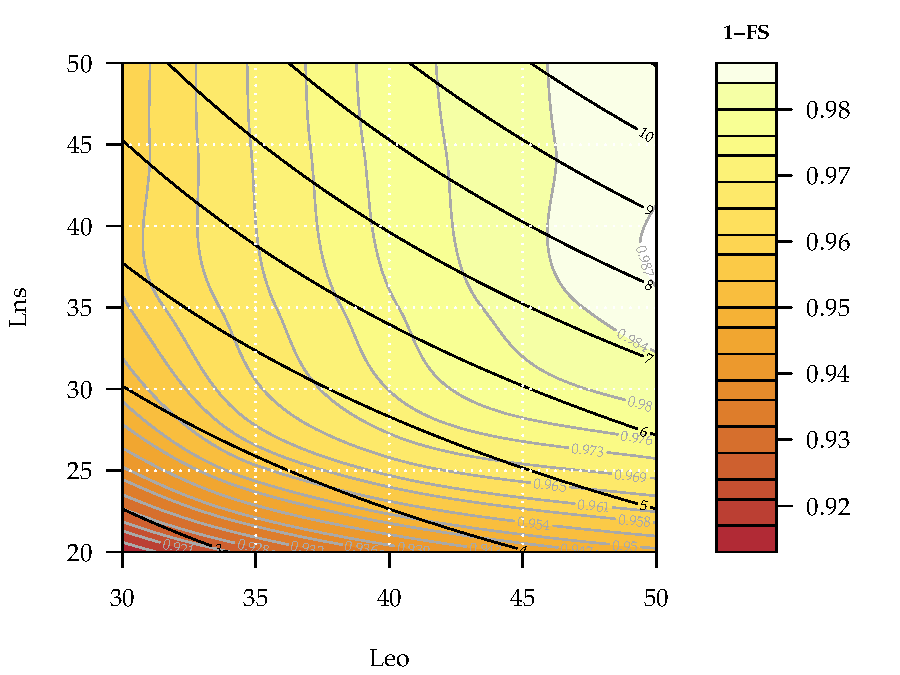
\includegraphics[scale=0.65]{../Figuras/AbacoSeguidor2X_Ene10}
\par\end{center}


\end{frame}

\begin{frame}[plain]
\frametitle{Ocupación de Terreno}


\framesubtitle{ROT para diferentes valores de Leo}
\begin{columns}[t]%{}


\column{4cm}

{\footnotesize \[
b=\frac{L}{W}=0.475\]
}{\footnotesize \par}


\column{4cm}

{\footnotesize \[
ROT=\frac{L_{ns}\cdot L_{eo}}{b}\]
}{\footnotesize \par}

\end{columns}%{}
\begin{center}
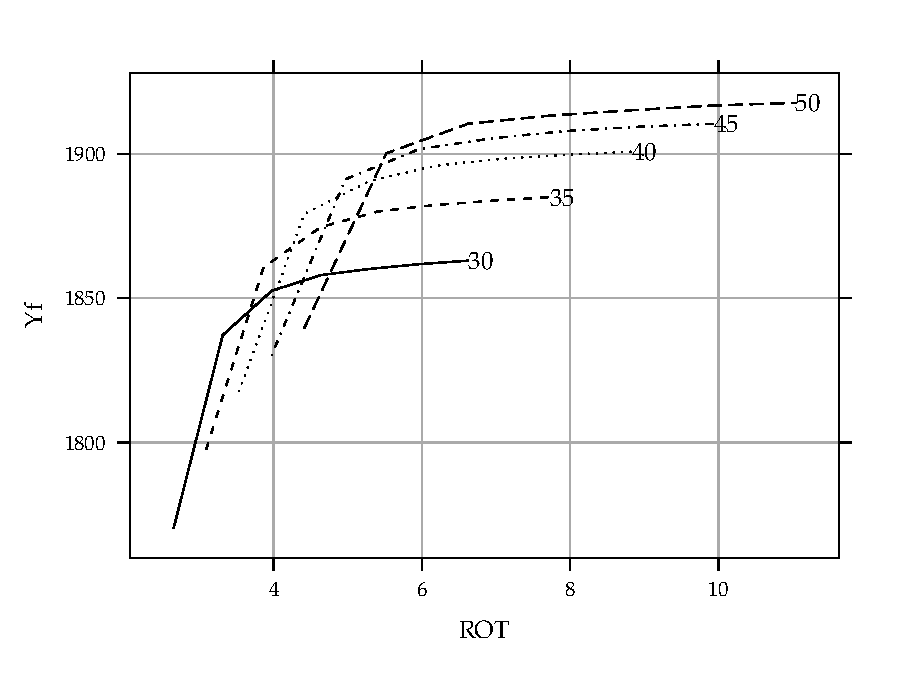
\includegraphics[scale=0.65]{../Figuras/AbacoSeguidor2X_Leo_Ene10}
\par\end{center}


\end{frame}

\begin{frame}[plain]
\frametitle{Ocupación de Terreno}


\framesubtitle{ROT para diferentes valores de Lns}
\begin{columns}[t]%{}


\column{4cm}

{\footnotesize \[
b=\frac{L}{W}=0.475\]
}{\footnotesize \par}


\column{4cm}

{\footnotesize \[
ROT=\frac{L_{ns}\cdot L_{eo}}{b}\]
}{\footnotesize \par}

\end{columns}%{}
\begin{center}
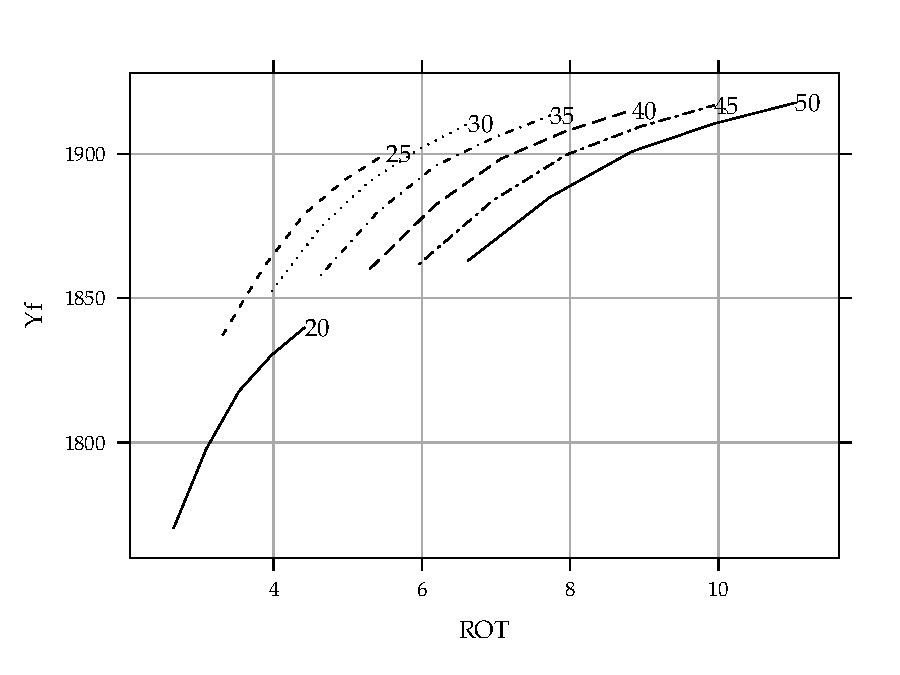
\includegraphics[scale=0.65]{../Figuras/AbacoSeguidor2X_Lns_Ene10}
\par\end{center}


\end{frame}


\subsection{Optimización: coste de la energía y sombras}
\label{sec:optimización}


\begin{frame}
\frametitle{Elección de separaciones}
\begin{block}
{Elección de separaciones}

La \textbf{separación óptima} entre elementos (seguidores o estructuras
estáticas) es aquella que conduce al \textbf{mínimo valor del coste
de la energía} producida por el sistema:
\begin{itemize}
\item Con mayor separación disminuyen las \textbf{pérdidas por sombreado
mutuo}, aumenta la productividad del sistema.
\item Con mayor separación aumentan los \textbf{costes relacionados con
el area ocupada} por unidad de potencia.
\item Con mayor separación aumentan los \textbf{costes relacionados con
los elementos de unión entre estructuras} (cableado, canalizaciones,
zanjas).
\end{itemize}
\end{block}

\end{frame}

\begin{frame}
\frametitle{Elección de separaciones}
\begin{block}
{}
\begin{itemize}
\item Esta separación óptima \textbf{depende} de las \textbf{estructuras
elegidas} y de las \textbf{condiciones económicas} de los elementos. 
\item La separación finalmente elegida debe \textbf{tomar en consideración
las condiciones del terreno} (fronteras, irregularidades, vaguadas,
etc.)
\end{itemize}
\end{block}

\end{frame}



\begin{frame}
  \frametitle{Radiación promedio}

  \begin{equation*}
    G_{ef, av} = 1/24 \cdot \left( 10 \cdot G_{ef,0} + 5 \cdot G_{ef,A}
      + G_{ef,B} + 2 \cdot G_{ef,C} + G_{ef,D} + 5 \cdot G_{ef,E} \right)
  \end{equation*}

  \begin{columns}

    \begin{column}{4cm}
      \begin{center}
        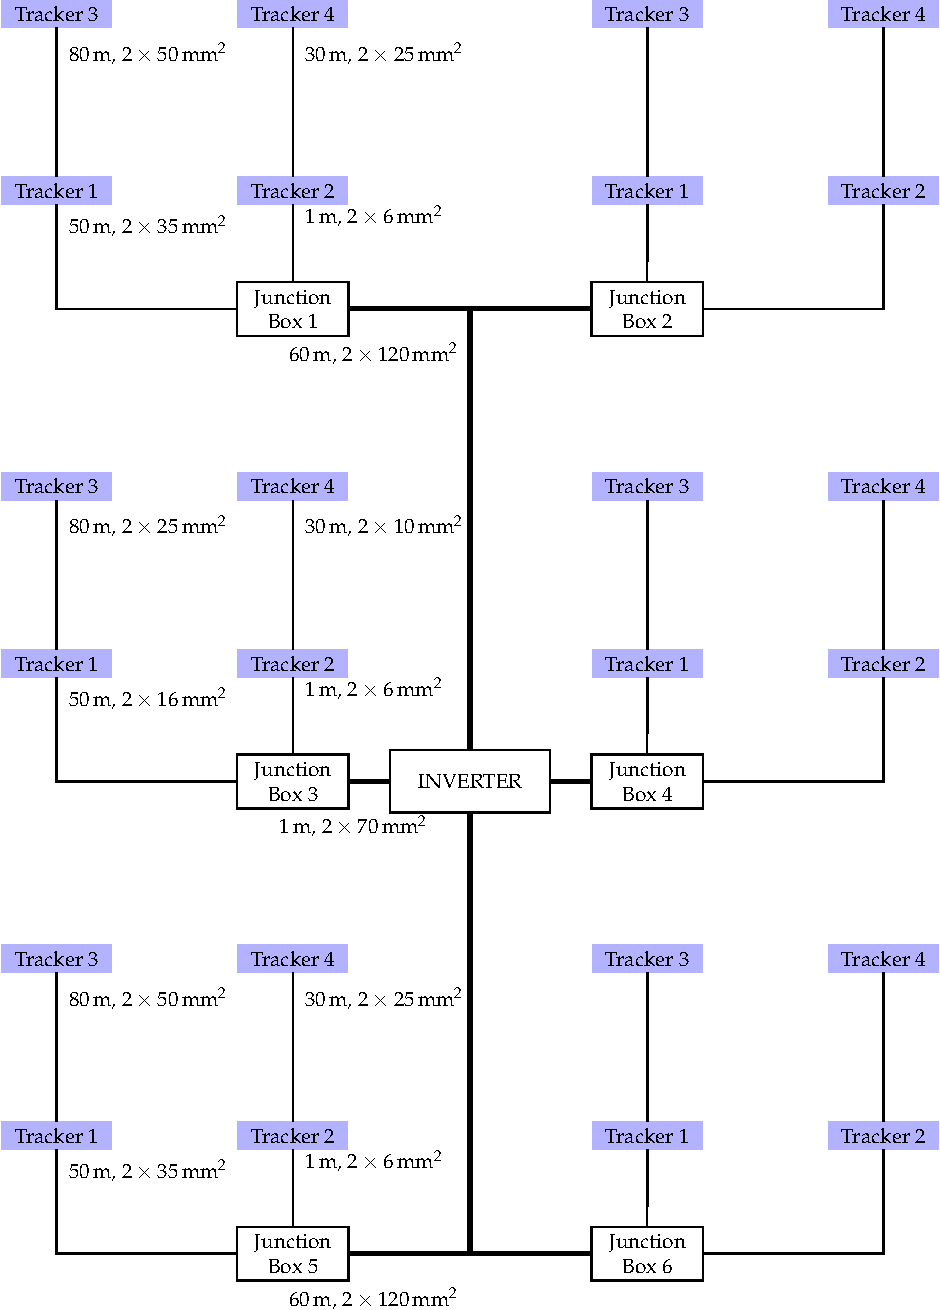
\includegraphics[scale=0.28]{../Figuras/plantConfiguration}
      \end{center}
    \end{column}

    \begin{column}{6cm}
      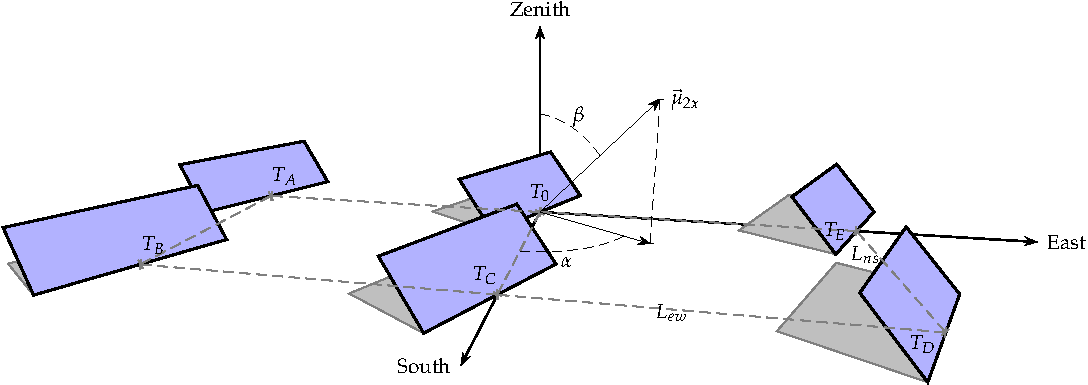
\includegraphics[scale=0.4]{../Figuras/6trackers}

    \end{column}
  \end{columns}


\end{frame}

\begin{frame}
  \frametitle{Cableado}

  \begin{center}
    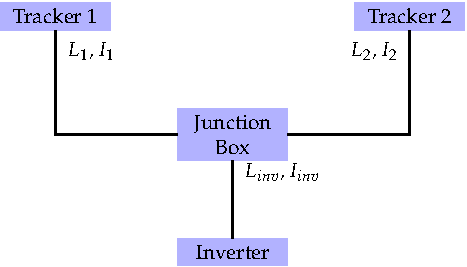
\includegraphics[scale=0.6]{../Figuras/wiring}
  \end{center}

  \begin{align*}
    \Delta U_{inv} &= \frac{\Delta U}{1+\sqrt{\frac{\sum_{i=1}^n
          L_{i}^2 \cdot I_{i}}{L_{inv}^2 \cdot I_{inv}}}} \\
    \Delta U_{inv} &+ \Delta U_i = \Delta U\\
    S_{inv} &= 2 \cdot \rho \cdot \frac{L_{inv} \cdot
      I_{inv}}{\Delta U_{inv}} \\
    S_{i} &= 2 \cdot \rho \cdot \frac{L_{i} \cdot I_i}{\Delta U_i}
  \end{align*}


\end{frame}

\begin{frame}
  \frametitle{Coste de la energía producida}

  \begin{align*}
    C_E &= \frac{C_P}{E_{AC}}\\
    C_p &= C_c + C_A + C_{PV}
  \end{align*}

  \begin{columns}
    \begin{column}{5cm}
      \begin{center}
        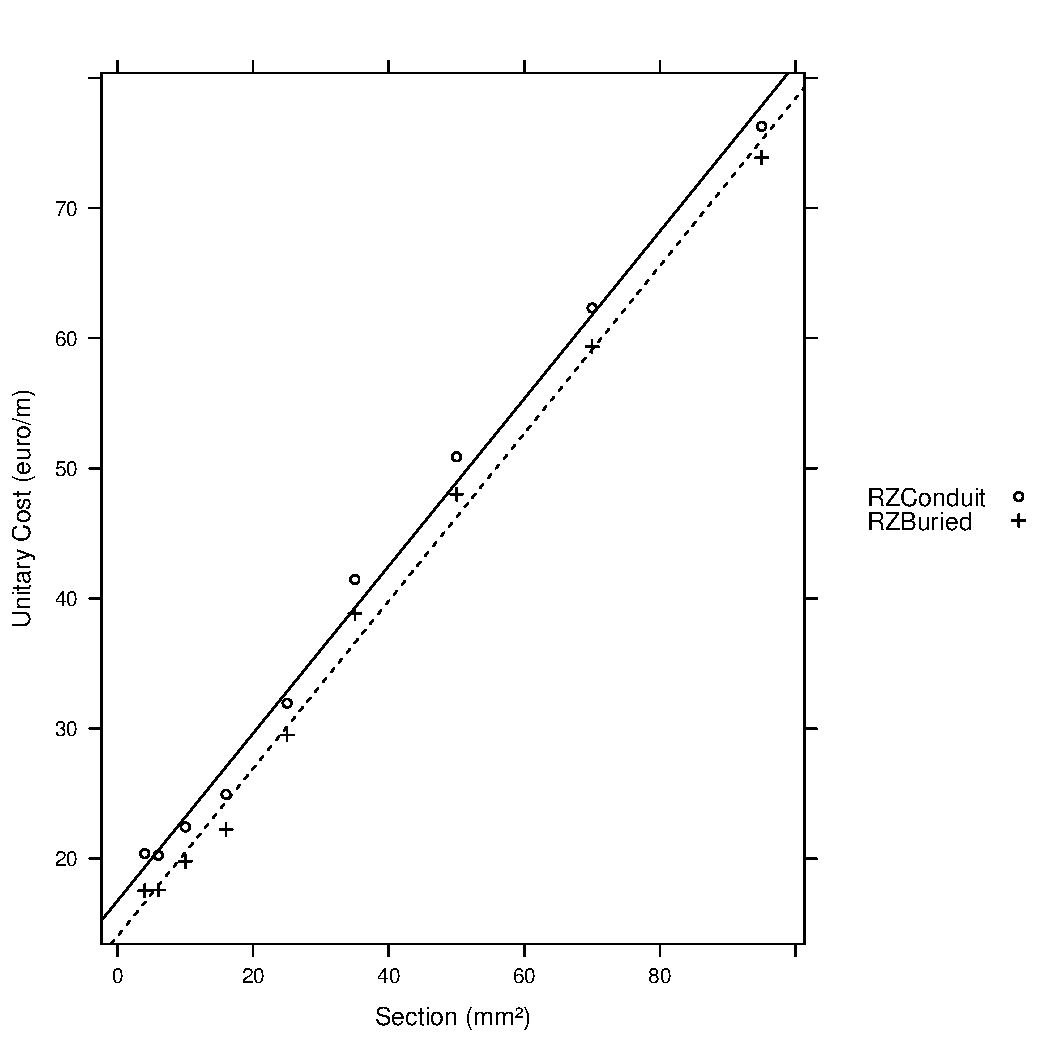
\includegraphics[scale=0.3]{../Figuras/WiringCosts.pdf}
      \end{center}
    \end{column}
    \begin{column}{5cm}
      $C_{PV}$ entre $\SI{2.5}{\text{\texteuro}\per\watt}$ y
      $\SI{5}{\text{\texteuro}\per\watt}$

      $C_A$ entre $\SI{1.5}{\text{\texteuro}\per\meter\squared}$ y
      $\SI{4}{\text{\texteuro}\per\meter\squared}$
    \end{column}

  \end{columns}



\end{frame}

\begin{frame}[plain]
%  \frametitle{Resultados}
  \begin{center}
      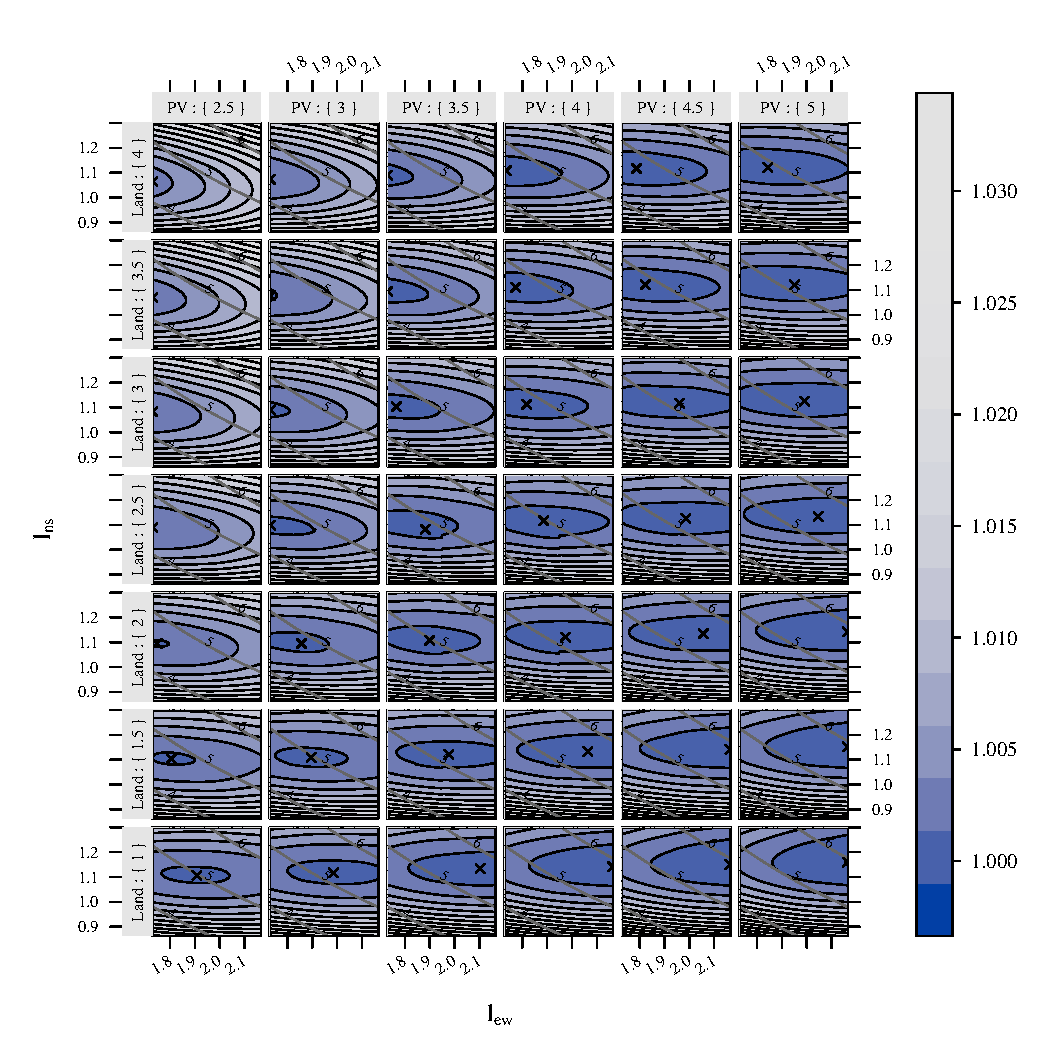
\includegraphics[scale=0.53]{../Figuras/matrix-300dpi}
  \end{center}
\end{frame}

\begin{frame}
  \frametitle{Resultados}
  \begin{center}
      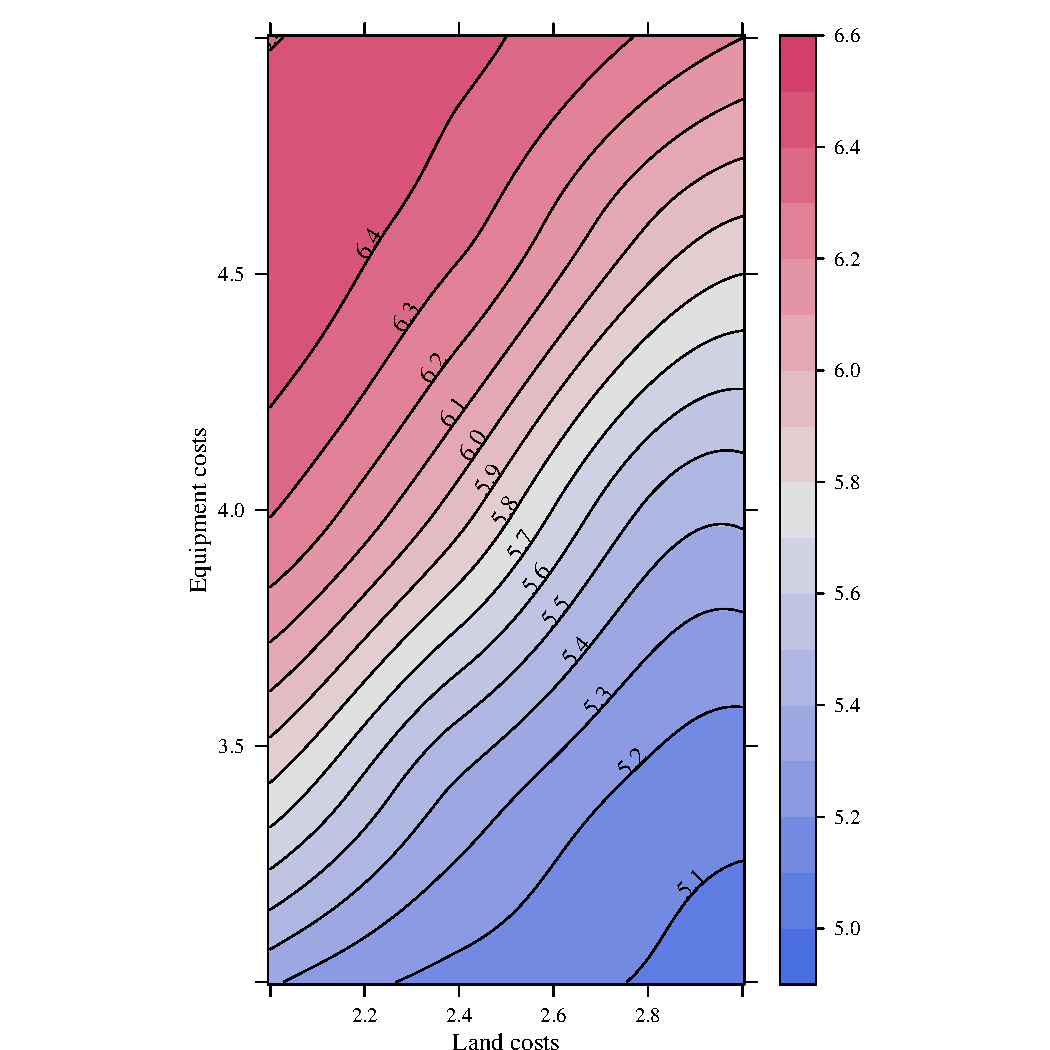
\includegraphics[scale=0.45]{../Figuras/GRRoptim}
  \end{center}
\end{frame}


\section{Resumen}


\begin{frame}
\frametitle{Resumen: Ocupación de terreno y productividad}
\begin{block}
{}

\begin{center}
\begin{tabular}{ccc}
\toprule 
SFCR & ROT & Productividad\tabularnewline
\midrule 
Estático & 2 & 1\tabularnewline
\midrule 
Eje Horizontal NS & 4 & 1,05-1,2\tabularnewline
\midrule 
Doble Eje & 6 & 1,3-1,5\tabularnewline
\bottomrule
\end{tabular}
\par\end{center}

\end{block}

\end{frame}

\end{document}
